% -*- root: These.tex -*-

\section{L'entrée de la simulation comme méthode pour les sciences sociales}

L'effort militaire Etats-Uniens a non seulement entrainé dans ses retombées le développement des outils informatiques mais aussi l'institutionnalisation d'entreprises de connaissances appuyées sur ces nouveaux outils tels que le MIT, ou dans un autre genre la RAND corporation, et autres diverses formations.

Ces institutions nouvelles ont largement contribué à susciter des rencontres interdisciplinaires qui vont favoriser la pénétration des idées de l'école néo-positiviste puis du paradigme systémique, jusque dans les sciences humaines et sociales.

\hl{CORRECT}
En parallèle, les lois de Boltzman pour la thermodynamique, ou le principe d’indétermination d'Heisenberg pour la mécanique quantique, viennent secouer le dogme du déterminisme scientifique hérité de la pensée mécanique, et plongent de nombreuses disciplines en \enquote{crises} \autocite[20-23]{Pouvreau2013}. Cette remise en cause est contemporaine de l'émergence d'une pensée \enquote{holiste} (ou pensée de la \enquote{totalité}) qui se construit en confrontation avec la démarche réductionniste classique.

C'est dans ce contexte que l'irruption de l'ordinateur (section \ref{sec:apparition_outil_informatique}) vient bouleverser en tout point le rapport des scientifiques aux données. Si les données de recensements focalisent les premiers travaux interdisciplinaires, les usages s'étendent rapidement à de nouvelles thématiques propres aux différentes disciplines. Un usage particulier de l'ordinateur va accrocher la curiosité de plusieurs chercheurs en sciences humaines et sociales. Cette capacité de celui-ci à supporter dans un environnement virtuel des expériences d'un genre nouveau, permettant de projeter des hypothèses dans le temps et dans l'espace pour observer l'évolution de systèmes dont on ne peut étudier leur comportement dans la réalité.

Afin de donner aux lecteurs des éléments de compréhension pour poursuivre la lecture du manuscrit, la partie suivante (section \ref{sec:apparition_simu_science_sociales}) expose quelques premières définitions générales sur les modèles et la simulation (section \ref{ssec:rapell_termes_generiques}) qui tiennent à la fois compte du contexte historique propre à leur apparition, mais s'intègrent également dans des grilles de classification plus récentes et volontairement plus englobantes, fruit des longs travaux menés par des épistémologues spécialistes de la simulation.

Après avoir constaté l'usage très ancien des modèles de simulation pour l'expérimentation, cet engouement sera précisé par la collecte de nombreuses références dans de multiples disciplines des sciences humaines et sociales (section \ref{ssec:engouement_sciencesociale}); autant de pointeurs pour qui voudra poursuivre ses recherches dans ce vaste océan bibliographique, dominé par de nombreuses références croisées du fait de l'interdisciplinarité et de la position centrale affichée par quelques auteurs.

En géographie la découverte des modèles de simulation coïncide avec l'établissement d'une véritable \enquote{révolution quantitative} (section \ref{sec:premier_modele_geo}), où l'usage de l'ordinateur accompagne, et rend possible même, cette transformation de la discipline voulue par une partie des géographes. C'est dans cette période 1960-1970 d'abondance des modèles (section \ref{ssec:revol_modele} ) que les premiers modèles de simulation émergent du fait de courants qui semblent diverger dans leurs intérêts : les planificateurs américains appuyés par la \textit{RAND corporation} \Anote{rand}, et les universitaires pionniers quantitativistes américains et suédois. L'occasion de voir ici quelle redéfinition des termes sont proposés par les géographes, et de présenter plus en détail les acteurs de ces deux courants de modélisation.

Il s'ensuit une crise de confiance envers les outils  (section \ref{sec:critiques_simulation}), et plus particulièrement envers la simulation, qui touche les disciplines des sciences sociales (section \ref{ssec:disciplines_touches}) à des dates, des degrés et pour des raisons très différentes. La géographie (section \ref{ssec:crise_mutation}), bien que touchée, elle aussi, dans le courant des années 1970 par des critiques sur ses outils, ses méthodologies, ses résultats présente toutefois dans ses rangs la présence des éléments actifs d'une transformation (auteurs, publications, etc.) qui laisse deviner pour les années suivantes un changement de paradigme explicatif sur lequel nous reviendrons plus en détail dans la section \ref{ssec:transition_annee70}. Un glissement plus qu'une rupture, qui ouvre de toutes nouvelles perspectives thématiques, méthodologiques et techniques aux futurs géographes modélisateurs. Ces mêmes modélisateurs qui apparaissent un peu partout sur la planète, faisant suite à l'essaimage de cette révolution à l'international. Les Français découvrent brutalement dans les années 1970 ce bloc de 15 années d'expériences - positives et négatives - acccumulées par les pionniers. On parlera donc plutôt ici d'une transformation que d'une véritable crise, les modèles de simulation n'ayant jamais réellement disparu de la discipline. 

\hl{CORRECT}
Cette transformation ne change rien toutefois aux différentes problématiques ayant fréiné l'adoption de la simulation dans de nombreuses disciplines, au contraire la \enquote{problématique de la Validation} qui en ressort se renforce même un peu plus avec la découverte de cette complexité à l'oeuvre dans les systèmes étudiés. Un facteur supplémentaire venant complexifier un peu plus les possibilités d'explorations de ces modèles, les méthodes algorithmiques et les capacités informatiques nécessaires s'avérant toute deux insuffisantes (section \ref{ssec:limitation_techniques_methodologiques}). Le chapitre \ref{sec:constante_problematique} traitera plus en détail les implications de ce dernier point avec des définitions et l'étude plus précise de cette transformation à l'oeuvre dans la façon de penser la construction des modèles de simulation.


%Ainsi malgré l'évolution et la démocratisation des outils informatiques et des plateformes de modélisation, l'accès à la ressource informatique (plateforme outils, formations limités, puissawnce disponibles) continue par la suite d'être un facteur limitant pour le développement de modèles plus complexes, mais aussi pour le calibrage et l'exploration efficace des comportements exprimés par ceux-ci, qui nécessite des compétences bien au delà du bagage technique initial des géographes. 

%Il manque l'écologie, cf unwin1992 121


\subsection{Irruption de l'outil informatique }
\label{sec:apparition_outil_informatique}

%GUllahorn cite le recueil 
%Supprime l'histoire du BIG DATA , qui est un anachronisme plutot >> 

L'accumulation et l'exploitation de données numériques sont des problématiques récurrentes pour les géographes et les sciences humaines en général. Ainsi depuis les années 1950-1960 les spécialistes de sciences humaines et sociales ont régulièrement signalé l'importance de l'outil informatique pour le traitement de leur données désormais informatisées, notamment depuis les premières grandes récoltes de données informatisées sur la population. \autocites{Kao1963, Hagerstrand1967b}[386]{Barnes2011}. 

On pourra citer à ce propos \textcite{Gullahorn1966} lorsqu'il pointe l'importance pour les sciences humaines et sociales du recueil \textit{Computer methods in the analysis of large-scale social systems} qui retrace les discussions issues d'un des tous premiers grands rassemblements interdisciplinaires organisés par le MIT. Cette conférence pilotée par un sociologue de la section \foreignquote{english}{Urban Studies} du MIT \autocite{Beshers1965} propose de faire le point sur les nouvelles méthodologies et techniques quantitatives et leurs utilisations dans les différentes disciplines en sciences sociales, avec cette volonté marquée de reprendre le contrôle sur la construction des modèles\Anote{ptvuebesher}, afin de faire face à ce qui apparaissait comme une manne de données nouvelles, les données américaines de recensement \textit{U.S Census}. Une question brûlante d'actualité à l'ère du \textit{Big data}, car cinquante ans après, et des centaines d'innovations techniques plus tard, peut-on enfin dire que les scientifiques ont pris le plein contrôle de leurs données et des outils associés permettant la construction des modèles ?

\begin{figure}[!htbp]
\begin{sidecaption}[fortoc]{\hl{CORRECT}Le \enquote{champignon informationnel} proposé par Frédéric Kaplan est révélateur de l'augmentation du champ d'expérimentation rendu possible par la numérisation des données (\textit{Digitization}), puis la simulation numérique (\textit{Simulated information}. Pour les données les plus anciennes, il est proposé d'extrapoler avec l'aide des historiens les informations très lacunaires dont on dispose pour reconstruire par simulation les données manquantes, et produire ainsi des scenarii historiques crédibles : \enquote{Par exemple, un carnet de bord d’un capitaine de navire vénitien nous indique bien plus qu’un itinéraire particulier, il nous informe sur les routes commerciales d’une époque. De la même manière, une gravure représentant une façade vénitienne nous décrit bien plus que ce bâtiment en particulier, mais nous renseigne sur les grammaires architecturales utilisées à cette époque particulière. Les historiens extrapolent très souvent de cette façon. Il s’agit simplement de formaliser et systématiser cette démarche.} \Anote{kaplan}}[fig:I_Champi]
 \centering
 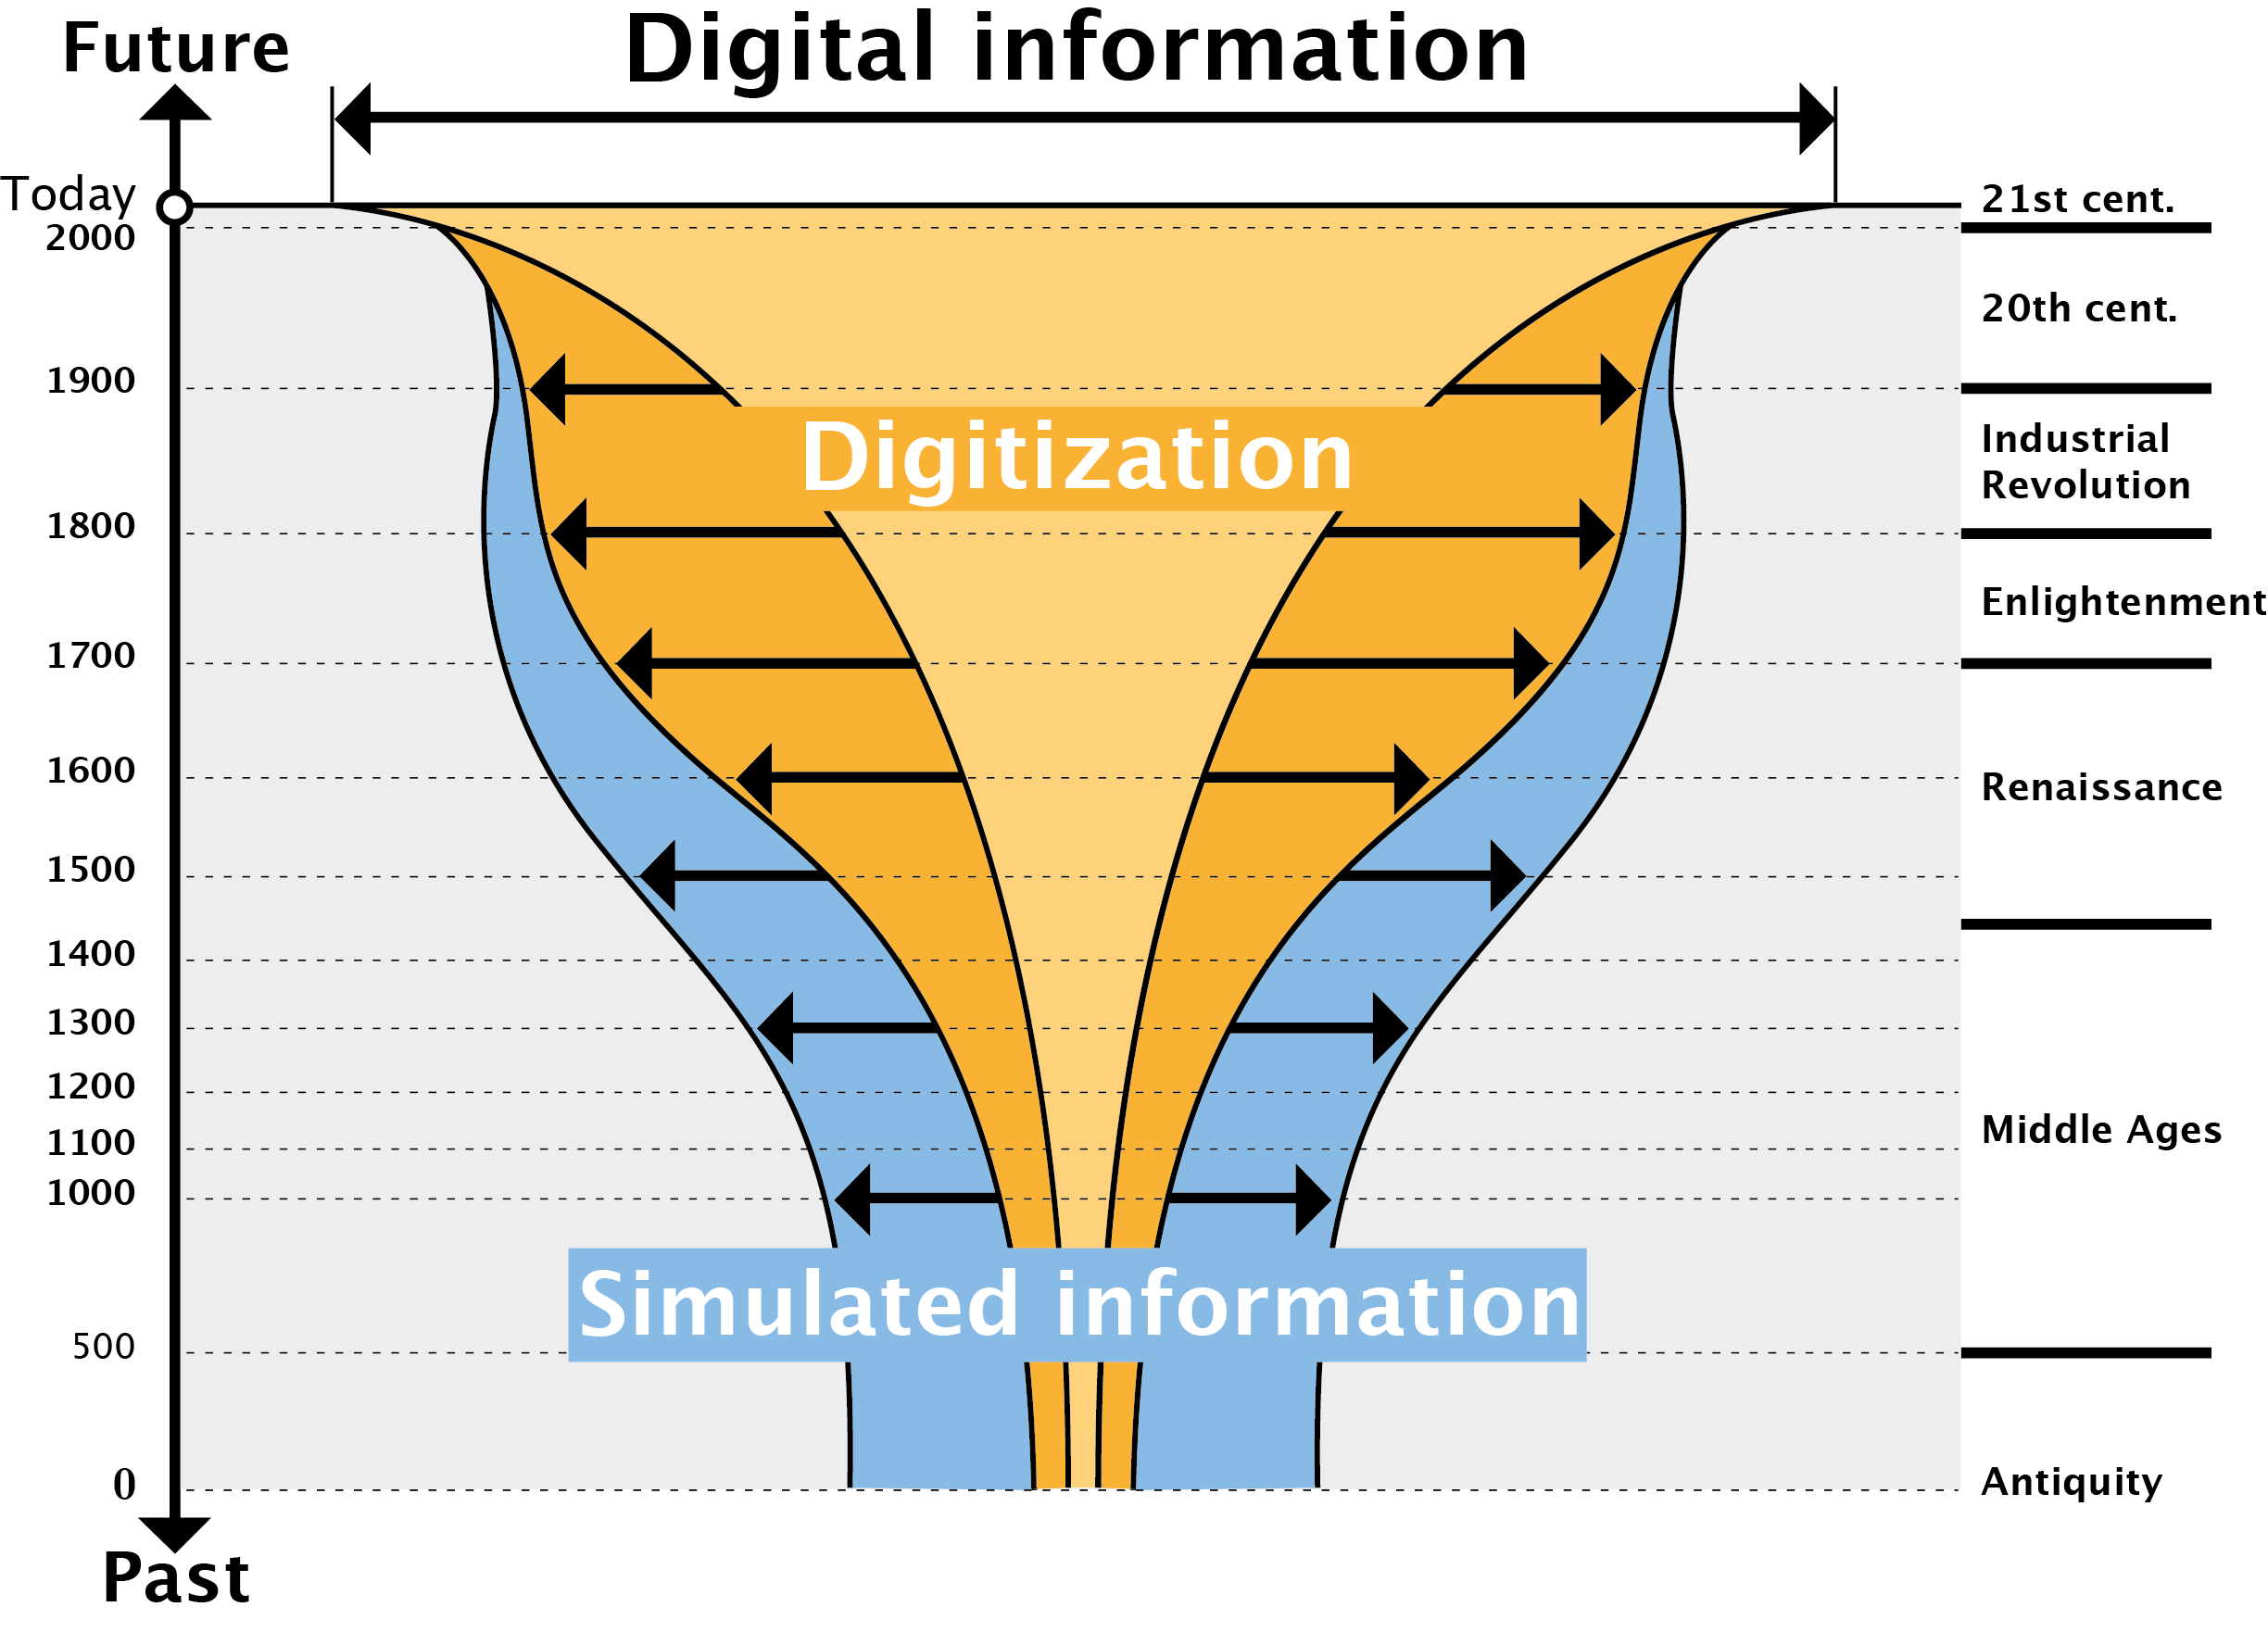
\includegraphics[width=.8\linewidth]{champignonKaplan.png}
  \end{sidecaption}
\end{figure}

Mais ce serait une erreur que de limiter l'application de ces nouveaux outils aux seuls stockages numériques récents, et ne pas citer l'importance du volume de connaissances accumulées ces derniers siècles par certaines sciences sociales telles que l'archéologie ou encore la géographie. Les lacunes dans l'information sont depuis longtemps une problématique récurrente pour de nombreuses disciplines en Sciences Humaines et Sociales. L'outil computationnel a permis, dès lors qu'il a été disponible, d'envisager de combler ces lacunes efficacement, comme tente de le résumer la figure \ref{fig:I_Champi} de Frédéric Kaplan. 

%\begin{figure}[tb]
%\raggedright
%\begin{sidecaption}{This is a subcaption just for illustration purposes. This is a subcaption just for illustration purposes. 
%Champignon Informationnel de Frédéric Kaplan. Page number is \LARGE\textbf{\thepage}}[fig:test]
%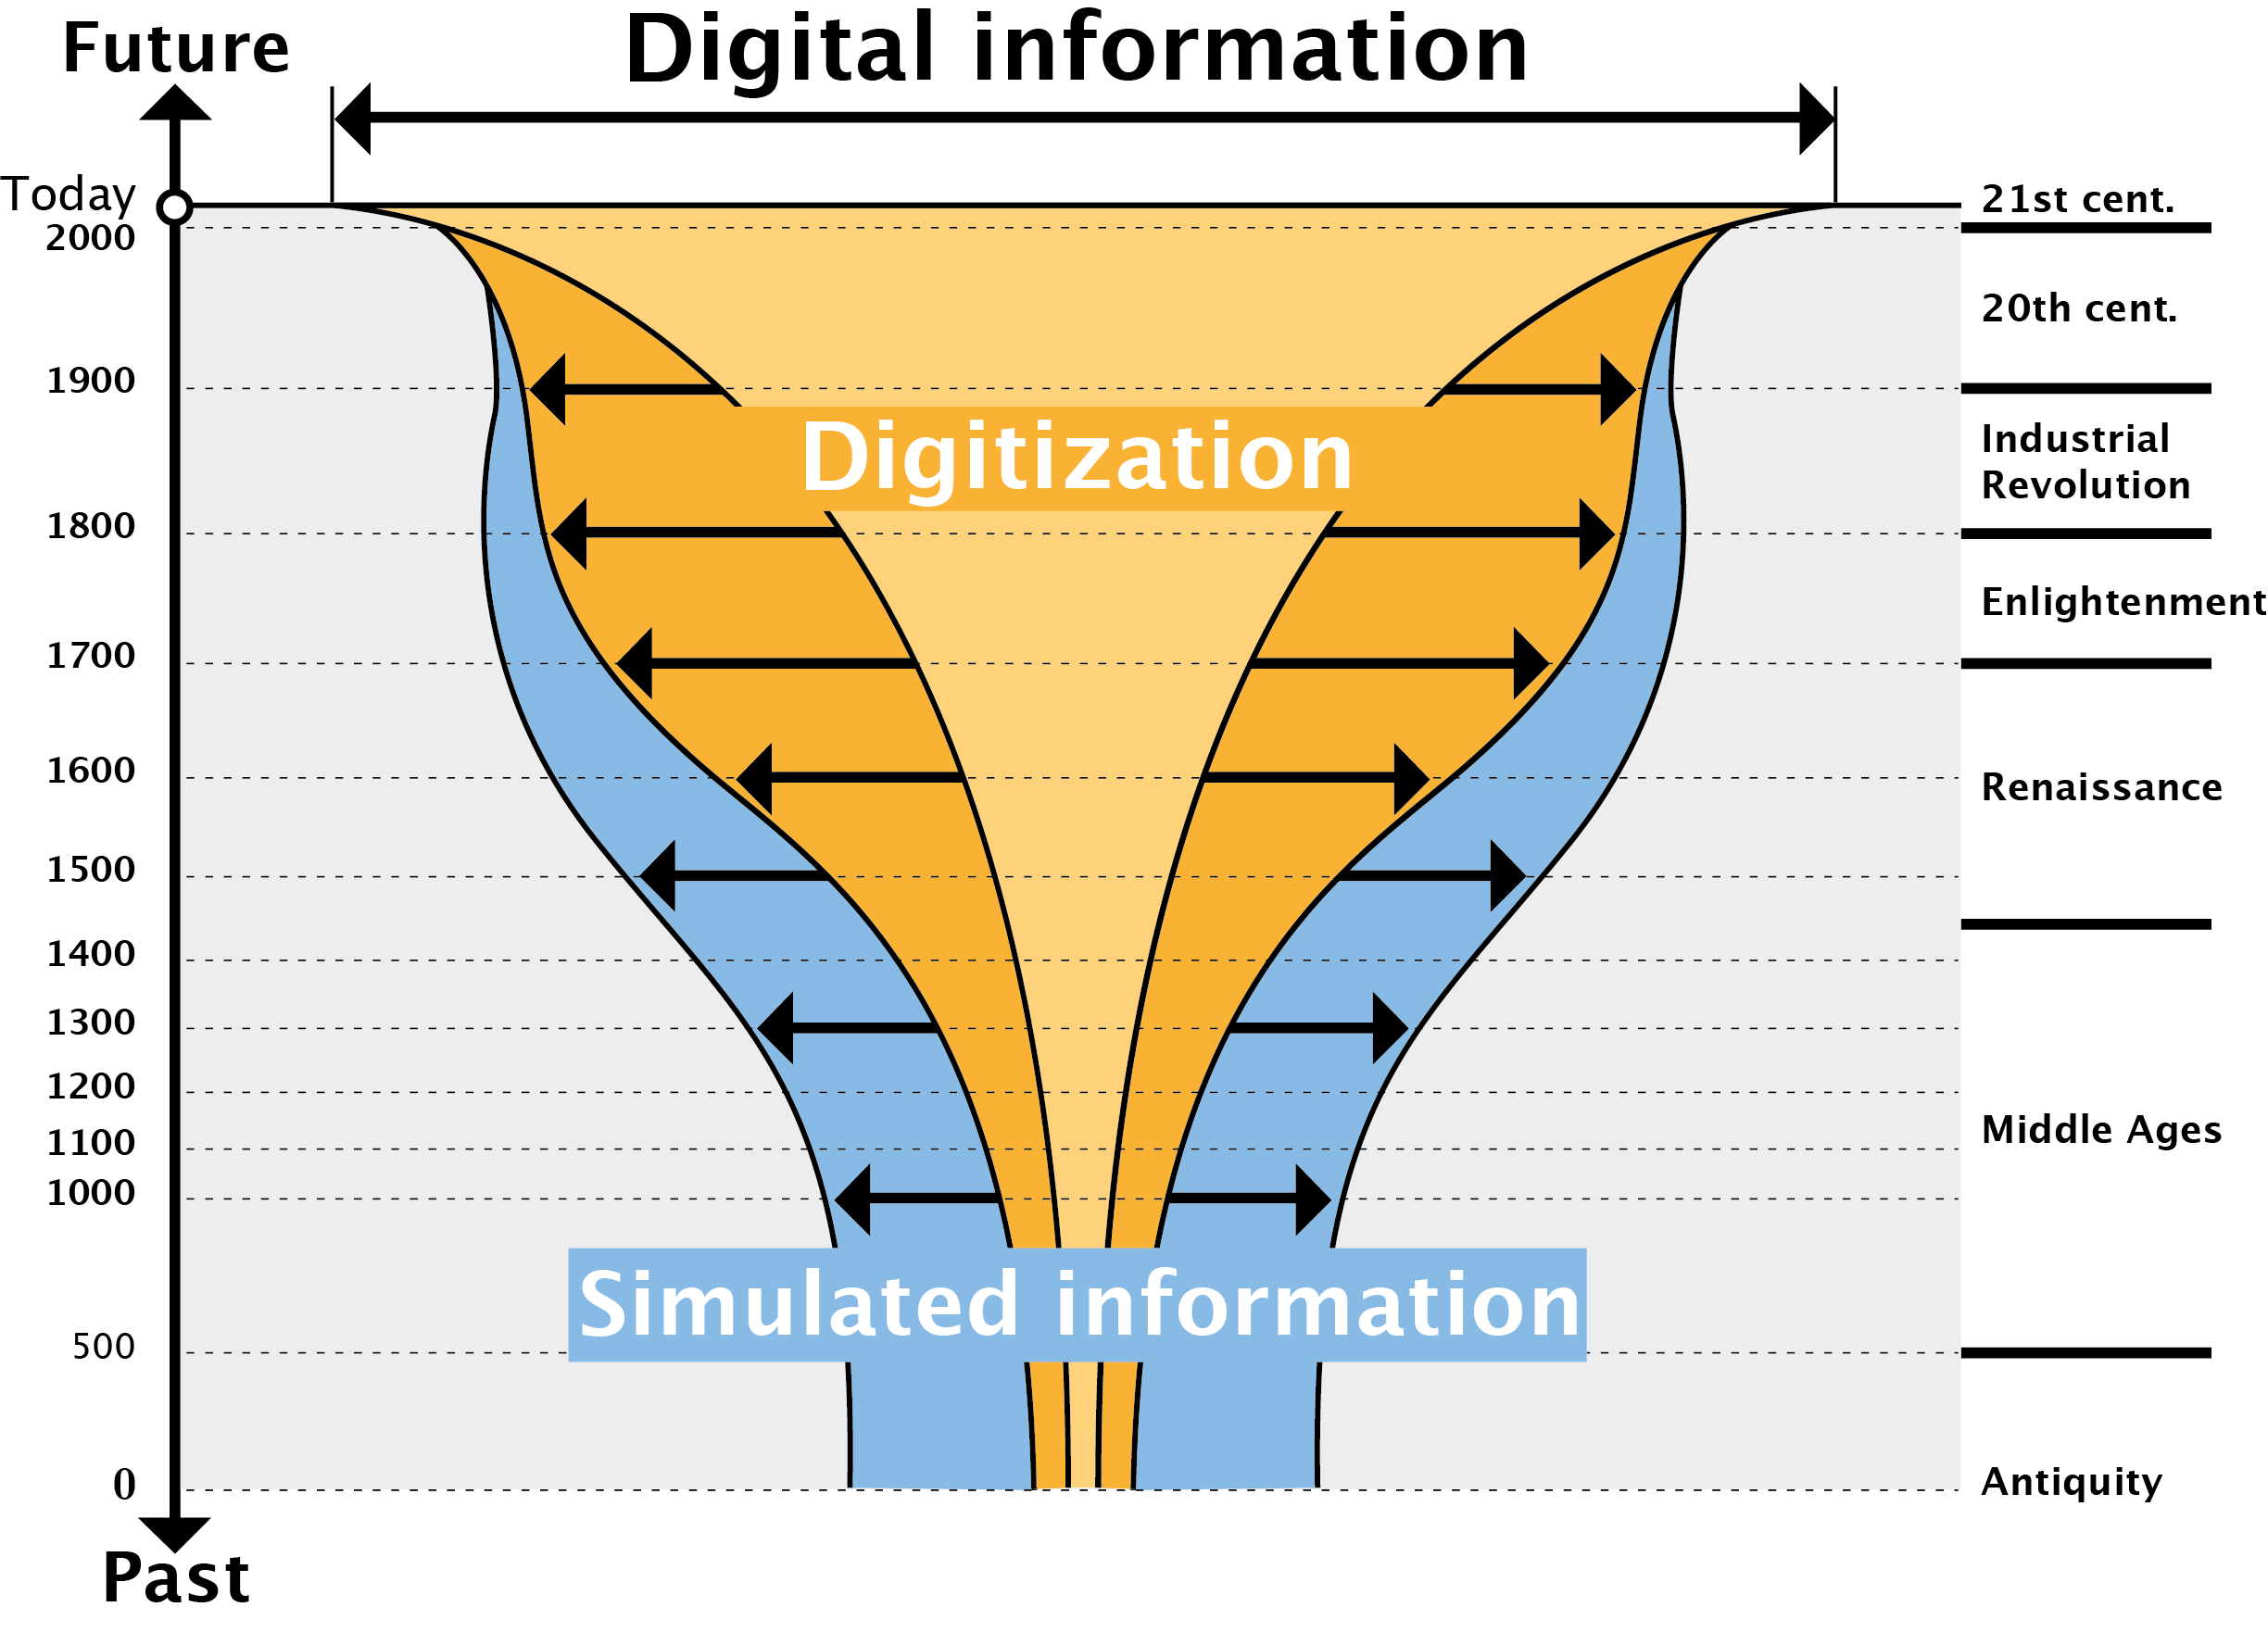
\includegraphics[width=\linewidth]{champignonKaplan.png}
%\end{sidecaption}
%\end{figure}

La classification automatique des données par l'ordinateur mais aussi la construction de modèles et leur simulation (au sens d'abord mathématique et parfois algorithmique du terme) apparaissent rapidement comme des enjeux pour la géographie. La simulation apparaît comme un outil de construction de connaissances absolument naturel et nécessaire pour confronter et construire les théories en rapport avec ces données \autocites{Kao1963, Hagerstrand1967b}. L'image de cette communauté interdisciplinaire agitant et confrontant ses problématiques méthodologiques, techniques, théoriques dans un but de progression commun, fait écho à des revendications plus récentes \footnote{On pensera notamment à la communauté ABM interdisciplinaire qui gravite autour de la revue JASSS fondée en  1990}. En réalité, cet esprit de partage tient d'une \enquote{volonté commune} qui apparaît quasiment avec l'apparition et la démocratisation des techniques de simulation. C'est ainsi que l'on trouve trace des efforts de cette communauté de chercheurs dans plusieurs ouvrages tels que \autocites{Borko1962,Beshers1965,Naylor1966,Dutton1971,Guetzkow1962,Guetzkow1972}.

Une citation d'un météorologiste du MIT, tout à fait remarquable par sa lucidité, anticipe ce qui sera le principal argument de l'emploi de la simulation en sciences humaines, à savoir un substitut à l'expérimentation.

\foreignblockquote{english}[\cite{Fleisher1965}]{I have argued that in the near future the social science will remain largely empirical and that simulation can serve as a device for making experiments \textbf{in vitro}. I think that this use is more important, at this time, than the massive making of models and that the principal contribution of simulation lies in the direction of intelligent, vivacious empiricism}

%Forrester1969 à ce sujet "In the social sciences failure to understand systems is often blamed on inadequate data... The barrier is deficiency in the existing theory of structure." \autocite[355]{Batty1976}

\subsection{Les conditions d'apparition de la simulation dans les différentes sciences sociales }
\label{sec:apparition_simu_science_sociales}

\subsubsection{Bref rappel autour des définitions de modèles et de simulations}
\label{ssec:rapell_termes_generiques}

Nous apportons ici une petite digression afin de préciser quelle acception de la simulation nous souhaitons mettre en oeuvre dans notre thèse.

\paragraph{Définitions générales du terme \enquote{modèle}}

\textcite{Varenne2013} ont entrepris une classification de la richesse historique associée aux termes de modèle et de simulation.

La première définition généraliste et aussi la plus couramment rencontrée dans la littérature est probablement celle de \textcite{Minsky1965} établie en 1965 : \enquote{ Pour un observateur B, un objet A* est un modèle d’un objet A, dans la mesure où B peut utiliser A* pour répondre à des questions qui l’intéressent au sujet de A } \autocites{Varenne2008}[15]{Varenne2013b}

A partir de cette définition très formelle, \textcite{Varenne2008} relève dans une analyse plus moderne du terme les cinq points suivants : 
\begin{enumerate}
  \item Le modèle n'est pas nécessairement une représentation.
  \item Le modèle doit son existence à l'existence d'un observateur subjectif, et d'un questionnement lui aussi subjectif.
  \item Le modèle est un objet qui a une vie propre, une existence autonome.
  \item L'existence du modèle est justifiée par l'existence d'une \enquote{fonction de facilitation}.
  \item Cette caractérisation minimale permet l'établissement d'une typologie.
\end{enumerate}

\textcite{Varenne2013b} propose dans des travaux plus récents d'associer à cette définition les travaux de Mary S. Morgan et Margaret Morrison qui replacent et caractérisent le rôle du modèle dans une enquête de connaissance par sa fonction de médiation (point 4 de la liste), une façon de faire écho à la problématique motivant la construction de modèles établis dans la définition de Minsky.

Un modèle est ainsi défini comme \enquote{\textit{un objet médiateur qui a pour fonction de faciliter une opération cognitive dans le cadre d'un questionnement orienté}, opération cognitive qui peut être de cognition pratique (manipulation, savoir-faire, apprentissage de gestes, de techniques, de conduites, etc.) ou théorique (récolte de données, formulation d'hypothèses, hypothèses de mécanismes théoriques, etc.)} \autocite[13-14]{Varenne2013b}

Les travaux actuels de \textcite{Varenne2008, Varenne2013b} dénombrent pas moins de cinq familles pour un total de vingt grandes fonctions, ce qui permet de situer efficacement la ou les problématiques - rien n’empêche les fonctions de se recouper - qui motivent la construction d'un modèle. 

Nous verrons dans la section \ref{ssec:revol_modele} que les géographes modélisateurs ont mis dans leur définition davantage l'accent sur le rôle et les résultats attendus des modèles, plutôt que sur ces aspects formels.

\paragraph{Définition générale du terme \enquote{simulation}}

Le terme \enquote{simulation}, tout comme le terme \enquote{modèle}, est porteur d'une polysémie \Anote{polysemie_simu} qui remonte aux alentours de l'accélération de sa diffusion en 1960, mais nous retenons ici simplement les acceptions qui concernent la simulation computationnelle.

Bien que la simulation apparaisse sous sa première forme computationnelle dans la technique de Monte-Carlo et les travaux de Stan Ulman, John Von Neumann, Nicholas Metropolis \autocites{Eckhardt1987, Metropolis1987}, il faut attendre les années 1960 et les avancées techniques nécessaires pour que son utilisation semble utile au plus grand nombre. L'historienne en économie \textcite{Morgan2004} estime que le mot se diffuse vraiment dans la communauté interdisciplinaire, et en économie, aux alentours de 1960. Elle souligne le rôle central de Martin Shubik, un des pères de la théorie des jeux \Anote{shubik_jeux} dans la construction de ce débat \Anote{shubick_sympo} autour de la notion, comme celui qui a servi à la fois d'intermédiaire important dans la rencontre entre les différents acteurs de l'économie expérimentale et de l'informatique, mais aussi comme celui tout aussi important de prospecteur au travers des vastes études bibliographiques qu'il a réalisées sur le sujet \autocites{Shubik1960a, Shubik1972,Morgan2004}.

Par la suite d'autres conférences et ouvrages vont proposer de délimiter, toujours dans une construction interdisciplinaire, cet objet \enquote{simulation}, comme on peut le voir dans \autocites{Guetzkow1962, Borko1962, Guetzkow1972, Dutton1971}. La simulation computationnelle est rapidement reconnue par les disciplines en sciences sociales ou les sciences du comportement comme un outil important pour la construction et l'extension de théories (\textit{theory-building} ou \textit{model-building} selon la fonction définie pour le modèle), de par sa capacité à manipuler certes des symboles mathématiques, mais aussi des symboles de plus haut niveau d'abstraction, propre à l'établissement de règle \autocite[924-925]{Clarkson1960}. Dans notre étude les modèles de simulation seront évoqués dans leurs dimensions avant tout numérique ou algorithmique (cf. dirigés par des règles) \autocite[36-38]{Varenne2013b}.

\subsubsection{La simulation vue comme laboratoire virtuel d'expérimentation, une analogie ancienne}
\label{ssec:labo_virtuelle}

Parmi la vingtaine de fonctions épistémiques recensées par \textcite[14-23]{Varenne2013b} motivant la construction de modèles de simulation, la caractéristique la plus souvent exprimée pour l'époque en sciences sociales est sûrement cette capacité à pouvoir \enquote{expérimenter} sur les modèles en mobilisant des processus et des interactions sélectionnés et animés dans le cadre d'une dynamique, d'un temps mimant celui des systèmes cibles \Anote{varenne_temps}, et cela même dans des conditions difficiles caractérisées par l'absence ou l'inconsistance des données, les expérimentations réelles impossibles ou difficiles, etc. mais pas seulement, car la simulation de modèles a aussi vocation à simplifier certaines simulations physiques coûteuses, ou trop limitées dans l'expression de nouvelles hypothèses. Ce lien entre simulation et expérimentation, complexe du fait de la relation entretenue entre le modèle et la réalité, est aussi ancien que la technique elle-même, Von Neumann affirmant dès le départ sa volonté de remplacer par des simulations sur ordinateur certaines techniques coûteuses de simulation physique \autocite[15]{Winsberg2013}.

Régulièrement employée dans la littérature, cette fonction d’expérimentation \Anote{laboVirtuel} revient également sous la forme de \enquote{laboratoire virtuel}, un terme qui prend selon les époques des teintes légèrement différentes, et cela quelles que soient les techniques sous-jacentes de support à la simulation des modèles.

Cette analogie ancienne entre simulation et laboratoire virtuel est illustrative d'une réalité dont on aurait bien du mal à nier l'existence tant celle ci est persistante dans cette littérature. Parfois le terme est invoqué directement, parfois il est implicite au discours présenté. Pour ne citer que quelques auteurs pionniers \Anote{legende_carnegie} dans l'historique de la notion, les premiers ouvrages collectifs en simulation et science sociale de \textcite{Borko1962, Guetzkow1962, Guetzkow1972} \Anote{ouvrage_1962}; les rapports et états de l'art des instituts scientifiques militaires américains \autocite{Harman1961}, et les travaux de Herbert Simon et Alan Newell \autocite{Newell1961}; et de façon plus localisé, en économie avec \textcite[915]{Shubik1960b}, en psychologie sociale avec \textcite{Abelson1968} \Anote{boudon_abelson}, le météorologue \textcite{Fleisher1965}, le couple d'Anthropologues/sociologues du comportement \textcite{Gullahorn1965}, l'archéologue anthropologue et informaticien \textcite{Doran1970}, la physicienne biostatisticienne et démographe \textcite{Sheps1971}, l'informaticien \textcite[3-4]{Forrester1971}, l'économiste informaticien \textcite{Naylor1966}, le professeur de science régionale \textcite[271]{Harris1966}, l'urbaniste \textcite[295]{Batty1976} sans oublier plus récemment \textcite{Epstein1996}, l'écologue \textcite{Grimm2006}, et encore sûrement bien d'autres auteurs. Une longue liste qui témoigne de l'intérêt pour cet outil bien au delà d'un simple critère de démarcation disciplinaire, technique, ou encore temporel; une hypothèse que nous allons développer par la suite.

\subsubsection{Un engouement pour la simulation qui touche l'ensemble des sciences sociales}
\label{ssec:engouement_sciencesociale}

Cet engouement pour la simulation de modèles touche toutes les sciences sociales ou presque. Nous dressons dans les paragraphes qui suivent une brève énumération des travaux qui en témoignent pour la période 1950-1970.

Suite au mouvement Cybernétique, à la convergence des travaux sur l'intelligence artificielle et les sciences cognitives, les premiers travaux qui visent la démonstration de la faisabilité de la simulation dans les sciences sociales viennent de Newell, Shaw, et Simon à la fin des années 1950 \autocite{Gullahorn1965} \Anote{gulahorn}. A ces travaux s'ajoutent ceux, en psychologie linguistique de l'équipe gravitant autour de \textcite[280-416]{Borko1962}, en psychologie des comportements sociaux de \textcite{Hovland1960}, d'\textcites{Abelson1961, Abelson1968} ou du couple \textcite{Gullahorn1965a} qui utilisent la simulation de modèles pour formuler, vérifier des théories sur la psychologie des individus et les modalités de leurs interactions avec les autres dans diverses situations \Anote{homonculus}, ce que \textcite{Ostrom1988} appellera \textit{a posteriori} les \foreignquote{english}{complex human processes}.

%La formation d’ingénieur de Coleman l’amène à prendre comme modèle un physicien : « My real hero is not Isaac Newton, but James Clerk Maxwell. He took Newtonian theory and developped from it a theory of gases, the Maxwell-Boltzmann distribution law of molecular velocities. I was fascinated by Maxwell because he was also concerned with the micro-macro problem. He had a very simple and neat theoretical framework of dimensionless molecules of any gas acting according to the law of motion, each with a certain mass and velocity. And from this he constructed a theory of gas. » (Coleman dans Swedberg, 1990, pp. 55-56).

En \textbf{sociologie}, la simulation émerge dans les années 1960-1970 selon \textcites[50]{Manzo2005}[16]{Manzo2007}, sous l'impulsion de pionniers dans la sociologie mathématique comme \textcites{Boudon1967, Gremy1971} en France \Anote{gremy} \Anote{boudon}, ou James Samuel Coleman aux Etats-Unis \Anote{columbia_coleman}. 

Celui-ci travaille sur des simulations liées à ses recherches sur l'éducation au début des années 1960 aux États-Unis, dont il a déjà publié des travaux dans l'ouvrage interdisciplinaire de \textcite{Guetzkow1962} en 1962, et qu'il publie ensuite \autocite{Coleman1965} dans une des premières revues abordant la méthode de simulation en sociologie, un numéro spécial des \textit{Archives Européennes de Sociologie} introduit par \textcite{Boudon1965} en 1965. Dans ce  numéro figure également une des premières publications de la simulation de diffusion d'\textcite{Hagerstrand1965} utilisant la technique de Monte-Carlo, un modèle qui recoupe les préoccupations du vaste courant interdisciplinaire dit des \textit{Social Network Analysis} (SNA) \autocite{Bernard2005}, qui touche tout autant aux structures de parenté (voir le paragraphe suivant pour des références en Anthropologie), qu'à la géographie (Hägerstrand à Lünd), ou à la sociométrie (modèle du sociologue mathématicien Coleman \textcite{Coleman1957}, mais également modèle de \textcite{Rapoport1961}, un biomathématicien de Chicago et cofondateur avec Boulding, Gerard et Von Bertalanffy de la société pour l'étude des systèmes généraux, ou GST) \Anote{lund_croisee}. Du point de vue français, outre l'analyse de Boudon sur ce sujet dans le numéro spécial de 1965, on trouve également une revue de ces mêmes avancées en simulation du côté de la sociologie politique (qui recoupe la psychologie sociale américaine), un état de l'art réalisé par \textcite{Padioleau1969} dans la \textit{Revue française de Sociologie} en 1969.

En \textbf{archéologie} \Anote{retrospective_archeo}, dans la très claire rétrospective historique faite par \textcite{Lock2003} en 2003 sur l'histoire de l'archéologie computationelle, l'auteur s'attache à bien séparer au moins deux sinon trois époques aux méthodologies et aux outils différents. En adoptant une posture un peu simplificatrice on peut donc affirmer que si l'archéologie pré-années 1960 se base principalement sur la récolte de données empiriques et la mise en exergue de \textit{pattern} dans ces mêmes données pour générer la plupart de ces explications, une rupture dans la discipline se dessine dès les années 1960-70 avec l'avénement d'un courant archéologique proclamant une \foreignquote{english}{New Archeology} (ou \textit{processualism}). Rejettant un empirisme beaucoup trop subjectif, celle-ci vante le retour à la seule \enquote{ Méthode Scientifique } pour générer des explications. 

Si la critique de \textcite{Binford1962} cristallise pour beaucoup cette rupture, 1967-1968 est également considéré comme une période particulièrement importante pour la structuration de ce courant dans la discipline. Des comptes-rendus \autocites{Cowgill1967, Whallon1972} et plusieurs publications phares, y compris en France \Anote{gardin} avec les colloques de Marseille et les travaux de Jean-Claude Gardin \autocites{Gardin1971, Dallas2015}, viennent souligner l'émergence progressive dans les années 1960-70 de nouveaux outils \Anote{caa} \Anote{retrospective_caa}, à la fois computationnels comme les statistiques \Anote{wilcock_stat} ou la simulation \autocite{Clarke1968}, ou plus conceptuels avec l'ancrage de la \foreignquote{english}{New Archeology} dans la pensée systémique \autocites{Clarke1968, Flannery1968, Binford1968} \Anote{archeo_systemique}. Des avancées qui fournissent un véritable support à ce changement des pratiques dans la discipline.

%\autocite{Binford1983}
Si \textcite{Binford1968,Binford1972} représente le point de vue américain, \textcite{Clarke1968} présente en Angleterre et à la même période (il est édité en 1968 par Binford) un point de vue un peu différent sur la \textit{New-Archeology}. Clarke est en effet sous l'influence des idées animant le campus de Cambridge, un haut lieu de changement ayant déjà accueilli une autre révolution, celle de la \textit{New Geography} \Anote{archeo_stat}. C'est dans cet environnement que Clarke publie en 1968 un premier livre \textit{Analytical Archeology} qui démontre le potentiel que pourrait avoir les statistiques spatiales, les modèles et la simulation stochastique en archéologie \autocites{Clarke1968, Clarke1972, Gardin1970}. Il est accompagné dans ses travaux par l'expertise, la volonté et les intuitions pionnières \Anote{doran_intuition} de \textcite{Doran1970} qui écrit également avec Hodson en 1975 l'ouvrage devenu référence \textit{Mathematics and Computers in Archaeology} \autocite{Doran1975} faisant état des travaux utilisant les toutes dernières techniques computationelles à la fois en traitement de données, et en simulation (Chaîne de Markov, Monte-Carlo, langage pour la simulation Dynamo, GPSS, etc.)

Ce militantisme qui semble recevoir un écho positif tout au long des années 1970, certains auteurs comme \textcite[38]{Whallon1972} n'hésitant pas à définir\Anote{whallon_simulation} la simulation comme un prolongement naturel à la pratique existante de construction des modèles. Cette mise en oeuvre de programmes pionniers se poursuit avec une diversification dans les usages jusqu'au début des années 80 et constitue une première phase d'appréhension de la simulation, plus qu'une adoption massive par la discipline \autocite{Lake2013}.

% VOir aussi Mathematics and Computers in Archaeology doran 1975, partie sur la simulation cf http://books.google.fr/books?id=ZAPvXcnz0kkC&pg=PA369&lpg=PA369&dq=The+computer+in+archaeology:+A+critical+survey+whallon&source=bl&ots=6et-F8jHab&sig=gQWgTIHRuO2ICqMJtrRdGovo9gs&hl=fr&sa=X&ei=OskxU5W5Nen20gW0_4DIDA&ved=0CGUQ6AEwBQ#v=onepage&q=whallon&f=false

%\autocite{Clarke1987}

A la croisée de plusieurs disciplines en sociologie, anthropologie et géographie on trouve les modèles de variation de population, ou modèles démographiques dont les hypothèses sont amenées à varier selon des facteurs biologiques, économiques, spatiaux faisant souvent appel à une dynamique des interactions humaines impossibles à expérimenter dans la réalité \Anote{sheps}. Dans cette branche se côtoient donc, macro-simulation, micro-simulation et modèles analytiques hérités des premiers démographes mathématiciens, comme le plus connu d'entre eux, Lotka dont les premières publications sur le sujet datent de 1907 \autocite[355]{Veron2009}.

%%FIXE CLEMENTINE : c’est intéressant, que la plupart des travaux pionniers que tu cites  apparaissent dans les urban studies.  Est-ce que c’est la ville qui est si complexe ou une dépendance au chemin des méthodes dans les champs d’études ? ou parce que urban studies est particulièrement interdisciplianaire que ça a dépasser les barrières des affiliations disciplinaires ?

C'est autour de l'économiste et - on l'oublie souvent - également ingénieur constructeur de machines analogiques Guy H. Orcutt \autocite{Watts1991} et les équipes de l'\foreignquote{english}{Urban Institute} que sont développés \autocite{Orcutt1978} plusieurs modèles pionniers de micro-simulation comme RIM (1969), TRIM (1973), ainsi que DYNASIM \Anote{plateforme_dynasim} entre 1969 et 1975 \autocites{Orcutt1957, Orcutt1960, Orcutt1976}. Pionnier d'une longue série de modèles de micro-simulation qui s'étend jusqu'à aujourd'hui \autocites{Merz1991, Merz1994}, ce concept va aussi inspirer différents modèles dynamiques en démographie avec les travaux de \textcite{Perrin1964}, \textcite{Sheps1971}, et \textcite{Ridley1966} avec REPSIM aux États-Unis, \textcite{Hyrenius1964} en Suède, \textcite{Horvitz1971} avec POPSIM, ou encore SOCSIM basé sur les travaux en anthropologie de \textcite{Gilbert1966}, qui viennent compléter efficacement les modèles analytiques inspirés des travaux de Lotka \autocite{Sheps1971}, père entre autres de la démographie mathématique moderne. On retient également l'inscription du pionnier \textcite{Sakoda1949} dans les développements des travaux sur la famille \autocite{Potter1966}, qui utilise le langage informatique DYSTAL qu'il a développé spécifiquement pour la simulation en science sociale \autocites{Sakoda1965, Lee1995}. Coïncidence de l'histoire, ou inspiration commune, Hägerstrand apportera de façon parallèle en géographie et dans la même décennie \autocites{Hagerstrand1952, Hagerstrand1967}, une vision micro similaire, à cela près qu'elle y ajoute un ancrage spatial des individus. 

Dans le cas de l'\textbf{anthropologie}, qui partage un tronc commun avec nombre de problématiques en archéologie et en psychologie, on retiendra le manuel édité par \textcite{Hymes1965} retranscrivant une conférence de 1962. Celui-ci contient deux articles importants pour la discipline, celui de \textcite{Gullahorn1965} et celui complémentaire de \textcite{Hays1965}. L'intégration de la simulation dans l'arsenal méthodologique prend part selon \textcite[274]{Bentley2009} d'un mouvement ayant pour objectif de mieux comprendre les contraintes sociales et culturelles dans les processus démographiques en général. Dans ce cadre par exemple de l'étude de la parenté ou \foreignquote{english}{kinship}, l'application de la simulation donne lieu à plusieurs expériences pionnières \autocites{Dyke1973, Dyke1981, Ruggles1993} en simulation comme celle de \textcite{Kunstadter1963}, mais aussi de \textcite{Gilbert1966}. Cet engouement continuera dans les années 1970 \autocite{Read1999} avec des simulations mettant en œuvre des processus stochastiques dynamiques comme par exemple dans les travaux de \textcite{Howell1978} et \textcite{Thomas1973}.

%\autocite{Costopoulos2007} . %Antony Wallace également, levy strauss 1955: les mathématiques de l'homme... 

%En utilisant la simulation non pas comme un solveur d'équation mais en utilisant la puissance des opérateurs symboliques à sa disposition pour la mise en temporalités de systèmes d'interaction dans des sociétés passées, Doran décrit une vision de la simulation qui n'est pas sans rapeller le multi-agent d'aujourd'hui. Une conception de la simulation reprise et concrétisée par DH Thomas en 1972.\footnote{La discussion sur  \href{www.jiscmail.ac.uk/cgi-bin/webadmin?A2=ind04\&L=simsoc\&F=\&S=\&P=39083} {@SimSOC}} 


% http://books.google.fr/books?id=G8sA95bz5pwC&pg=PA143&lpg=PA143&dq=%22Social+Physics%22+stewart+cybernetics&source=bl&ots=FsOC2mqHvr&sig=cS914G7pelGvgG6bG32fKsmWWPc&hl=fr&sa=X&ei=yTRAU5m7OIOH0AXwtYEY&ved=0CDsQ6AEwAQ#v=onepage&q=%22Social%20Physics%22%20stewart%20cybernetics&f=false
% "Social Physics" stewart cybernetics
% http://www.eoht.info/page/Princeton+Department+of+Social+Physics
% http://books.google.fr/books?id=F84mS2nnjWsC&pg=PA105&lpg=PA105&dq=geographer+reino+ajo&source=bl&ots=buVSBElr7Y&sig=_NXU0Py2goM2c6fVi1To3dUwqHQ&hl=fr&sa=X&ei=0DBAU_niJqrO0AWk44CwCw&ved=0CG8Q6AEwBw#v=onepage&q=geographer%20reino%20ajo&f=false
% http://www.persee.fr/web/revues/home/prescript/article/ingeo_0020-0093_1957_num_21_5_6491_t1_0223_0000_5#
% http://www.eoht.info/page/Social+physics
% Contributions to "social Physics" reino ajo
% Stewart, J.Q. "The Development of Social Physics"

\subsection{Les premiers modèles de simulation en géographie}
\label{sec:premier_modele_geo}

\subsubsection{Une \enquote{révolution quantitative} au cœur de multiples convergences}
\label{ssec:revol_quanti}

L'apparition et la diffusion de ces techniques quantitatives n'est pas le résultat d'une convergence unique, mais bien d'une succession de moments dont la fréquence et l'étalement temporel est difficile à cerner et empêche sur ce sujet toute exhaustivité. 

On retiendra toutefois plusieurs grands facteurs, à la fois généraux, et d'autres plus spécifiques à la géographie, dont certains qui peuvent paraître étonnamment antinomiques. Une convergence qui s'illustre dans la richesse et la diversité des transformations qui touchent la discipline géographique entre 1950 et 1970, un constat déjà établi par bien d'autres auteurs \autocite{Varenne2014}

%[28-29]Claval2003
%http://books.google.fr/books?id=s5xjIsejTjkC&pg=PA28&lpg=PA28&dq=h%C3%A4gerstrand+positivism&source=bl&ots=FrIMA95glO&sig=9Knqs1cLfJJefcc30qwsIMDzW-s&hl=fr&sa=X&ei=UMVDU86hJ-mS1AWPmIDoCw&ved=0CC4Q6AEwADgK#v=onepage&q=h%C3%A4gerstrand%20positivism&f=false

\paragraph{L'influence de l'école néo-positiviste}

Le néo-positivisme, néo-empirisme, positivisme logique selon les étiquettes, est un mouvement philosophique important, sinon peut-être le plus important, entre les deux guerres. Ce cercle dont on trouve les premières traces dans les années 1908 à Vienne, est organisé autour de grands débats, dont la caractéristique est d'être fréquentée par un grand nombre d'intellectuels, issus de plusieurs disciplines. Tout au long de son évolution caractérisée par différentes phases (avec une apogée durant la troisième phase entre 1928-1934), de multiples courants d'opinions \textcite[126]{Ouelbani2006} vont être amenés à se côtoyer, du fait des débats internes, mais aussi des critiques extérieures au cercle. C'est donc à ce titre que \textcite[11]{Ouelbani2006}, préfère parler de \enquote{programme néo-positiviste} \Anote{ouelbani_positivisme} plutôt que d'un réel courant unifié.

Inspirés des sciences naturelles, et plus particulièrement d'une observation des sciences physiques et mathématiques, les tenants du programme néo-positiviste sont motivés par l'unification des sciences et pensent l'application d'un tel programme incontournable pour fonder des sciences sociales véritablement \enquote{scientifiques} \autocite[1-20]{Ouelbani2006}. 

Les positivistes logiques ont ceci de particulier qu'ils raisonnent sur des démonstrations logiques encapsulant les énoncés observationnels décrits dans une logique formelle qu'ils veulent non ambiguë. Entre empirisme et logicisme, ce programme réductionniste \Anote{carnap} fait porter toute la connaissance sur l'expérience; ce qui mène avec l'aide de l'analyse logique et mathématique à l'élimination de toute métaphysique, et de toute structure a priori (anti-kantien) dans la construction des énoncés d'observation. Ainsi l'inférence déductive se fait seulement sur des énoncés d'observations qui sont \textit{a posteriori} tout à fait justifiables et donc mobilisables dans celles-ci seulement s'ils sont cohérents.

Selon le géographe épistémologue Olivier Orain \Anote{cour_orain}, \textcite{Hacking1989} a très bien saisi ce qui fait les axes communs des différentes relectures du terme positivisme. 

\blockquote[{\cite[82]{Hacking1989}}]{Le positivisme peut se définir par quelques idées forces. \begin{enumerate*}[label=(\arabic*)] \item L’importance accordée à la vérification (ou à une variante comme la falsification) : une proposition n’a de sens que si l’on peut, d’une quelconque manière, établir sa vérité ou sa fausseté. \item La priorité accordée à l’observation : ce que nous pouvons voir, toucher ou sentir fournit, sauf pour les mathématiques, la matière ou le fondement le plus appréciable de la connaissance. \item L’opposition à la cause : dans la nature, on ne trouve pas de causalité dépassant ou surpassant la constance avec laquelle des événements d’un certain type sont suivis par des événements d’un autre type. \item Le rôle mineur joué par l’explication : expliquer peut contribuer à organiser des phénomènes mais le pourquoi reste sans réponse. On peut seulement remarquer que le phénomène se produit régulièrement de telle ou telle manière. \item Opposition aux entités théoriques : les positivistes ont tendance à être non réalistes parce qu’ils limitent la réalité à ce qui est observable mais aussi parce qu’ils s’opposent à la causalité et se méfient des explications. Leur rejet de la causalité les fait douter de l’existence des électrons simplement parce que ces derniers ont une action causale. Ils soutiennent qu’il s’agit là seulement de régularités constantes entre phénomènes. \item L’opposition à la métaphysique est finalement le dénominateur commun entre les points (1) à (5) ci-dessus. Propositions invérifiables, entités inobservables, causes, explications profondes, tout cela, dit le positiviste, est objet de métaphysique et doit être abandonné.\end{enumerate*}}

Une parenté qui dans le cas du programme néo-positiviste est difficile à isoler tant l'acceptation par les proches (comme Popper) ou membres du programme (certains préféreront même le terme empirisme logique) est amenée à varier. pour en savoir plus sur ce sujet, on pourra se référer à cette classification proposée par \textcite[81-86]{Hacking1989}.

L'apogée du groupe à Vienne est de courte durée, avec les pressions du régime nazi et l'annexion de l'Autriche, le groupe est dissous. De nombreux acteurs du mouvement sont alors contraints à l'exil et nombreux sont ceux qui vont aux États-Unis. A ce moment-là, ce programme philosophique est alors quasiment inconnu des philosophes pragmatistes américains, mais paradoxalement il va trouver un très bon accueil sur ce nouveau territoire.

C'est sur cette philosophie pragmatique depuis longtemps installée (Peirce, Dewey) que vient se greffer ce nouveau programme, jusqu'à finalement quasiment l'éclipser. Un transfert que l'on n'imagine pas totalement unilatéral, et il est presque évident que le discours originel viennois tire largement profit d'une philosophie pragmatiste compatible dans ses fondements \footnote{ Ainsi selon \textcite[149]{Ouelbani2006} Carnap aurait été rassuré en 1935, date de son arrivée aux Etats-Unis, \enquote{ [...] de trouver une ambiance philosophique différente,en ce sens que les jeunes philosophes étaient intéréssés par des méthodes scientifiques et logiques}}. C'est ce que \textcite[123]{Wilson1995} affirme en disant que les pragmatistes \foreignquote{english}{[...] had created the conditions in which logical positivism and other analytic philosophies could flourish and ultimately displace them as the dominant voice in mid-century philosophical debates} mais aussi les conditions de son dépassement \foreignquote{english}{Pragmatism, then, not only created the conditions in which logical positivism and analytic philosophy could flourish in the United States, it also contained the seeds of the postanalytic philosophies that have attempted to move beyond [...] }. Ce programme va se diffuser à la fois sur les bancs des universités, mais aussi via les grands instituts scientifiques après-guerre qui font publicité de cette science \foreignquote{english}{mainstream}, organisée aux Etats-Unis autour de l'ordinateur. 

La RAND fait partie de ces instituts fondés après-guerre qui approchent dès 1947 les sciences sociales \autocite{Rand106} et n'hésitent pas à mettre en avant par la suite les stars de la philosophie positiviste de l'époque comme Reichenbach \autocite[384-385]{Barnes2011} .

\paragraph{L'apparition de mouvements interdisciplinaires fédérateurs}

L'apparition de grands mouvements de convergence interdisciplinaires et leur intérêt pour l'application de nouveaux concepts et techniques aux sciences sociales, dont certains prennent par la suite la forme de paradigme du fait de leur portée d'application : Cybernétique de Wiener, \textit{projet} de la \foreignquote{english}{General System Theory} de Bertalanffy \autocite[9]{Pouvreau2013} s'organisent autour de grandes structures de recherches comme le MIT, la RAND, qui favorisent les collaborations par la mise en place d'équipes de travail pluridisciplinaires.

Parmi les ramifications directes de ces coopérations, on citera par exemple la \foreignquote{english}{social physics} de \textcite{Stewart1947}. Du fait des liens développés à l'université de Pennsylvanie, lieu de ses études et siège de la fondation de la science régionale d'Isard en 1954, Stewart sera amené avec sa rencontre avec Warntz, un géographe atypique qui plonge très tôt dans l'interdisciplinarité, à publier dans la revue \textit{Regional Sciences} \autocite{Stewart1958}.

Les retombées de ces interactions sur la géographie sont importantes \Anote{systemique_sousjacente}, et fournissent tout autant \begin{enumerate*}[label=(\alph*)] \item des concepts généraux en correspondances avec les débats qui animent l'ensemble des sciences (sensibilités aux conditions initiales, équifinalité, bifurcation et catastrophe, boîte noire, rétro-causalité, hiérarchie d'emboîtement, etc.), \item un catalogue d'isomorphismes \Anote{isomorphismes} supplémentaires dont la correspondance reste à évaluer dans notre discipline \autocite{Wilson1969}, \item  une méthodologie et une typologie des modèles tirés de la recherche opérationnelle \autocite{Ackoff1962} \Anote{or_bertalanffy} et largement revendiqués par les géographes dans la décennie 1960-70, un constat tiré de la lecture d'états de l'art \autocite{Kohn1970}, ou d'ouvrages phares sur le sujet comme ceux de \textcites{Berry1964a, Haggett1965}, \item la découverte d'une science mathématique des systèmes dynamiques en correspondance avec ces nouveaux concepts, accessibles soit par un vocabulaire graphique opérationnalisable (DYNAMO, STELLA) \autocite{Forrester1961}, soit par des langages de programmation tout à fait traditionnels \autocite[304-305]{Batty1976} ! \end{enumerate*}

On citera parmi les pionniers d'une exploration volontaire de cette convergence en géographie, \textcite{Haggett1965} en 1965, \textcite{Chorley1962} avec la géomorphologie en 1962 , \textcite{Berry1964a} avec les villes en 1964. 

\paragraph{Les influences des \enquote{passeurs de modèles}}

Ces influences se sont réalisées à l'échelle internationale par Torsten Hägerstrand, Edgar Kant \Anote{footnote_kant}, Christaller et Lösch \autocite[119]{Berry1970}, ou dans un cadre plus national avec le travail de traduction ou de mise à disposition de textes originaux par les économistes et géographes Lösh, et Isard.

\paragraph{La conjoncture politique favorable}
% tous de chicago ? 
L'impact de la conjoncture politique et l'importance de grands \textit{Think-Tank} comme la RAND, et du MIT qui remobilisent en sortie de guerre des armées d'ingénieurs alors désoeuvrés sur des missions plus scientifiques. On soulignera à la même période le rôle joué chez les géographes de Chicago \autocite{Harris1979}, Edward Ullmann \autocites{Ullman1941, Harris1977, Glick1988}, Chauncy Harris \autocite{Harris1945, Lichtenberger2005} et Edward Ackerman \autocites{Ackerman1958, Ackerman1963} dans la transformation institutionnelle de la géographie, dont la qualité en tant que corps de métier a pu être remarquée en temps de guerre. Cela se traduit sur la durée par un financement de la marine (\textit{Office Of Naval Research}), qui profite aussi de la nouvelle \textit{Regional Science} fondée par Isard. On trouvera plus d'informations sur ces inter-relations entre instituts après-guerre et leur impact sur l'établissement d'une géographie quantitative dans les publications de \textcites{Barnes2006a, Barnes2008}.

\subsubsection{D'une révolution quantitative à une révolution des modèles}
\label{ssec:revol_modele}

De cette \enquote{révolution quantitative} aux origines on le voit multiples, certains auteurs préfèrent ne retenir qu'une certaine essence de cette volonté nomothétique. Cette \enquote{révolution des modèles} comme préfère en parler \textcite{Wilson1970, Varenne2014} fait ici écho à cette déferlante de modèles qui apparaissent dans la décennie 1960-1970, et dont on trouve un recensement quasi exhaustif dans plusieurs ouvrages de référence \autocite{Haggett1965,Chorley1967}.

Une fois révélée cette profusion d'approches sous jacentes à l'emploi, parfois confus, d'un même terme, s'ensuit chez les géographes une tentative de classification, de définition de cette pratique de modélisation. Il en ressort des typologies, l'évocation de divers substrats ( analogique, iconique, symbolique ) la plupart du temps empruntés dans les ouvrages de spécialistes alors disponibles. Ainsi, les deux sources d'inspirations de \textcites[106]{Berry1963}{Haggett1965} sont à ce moment-là des références issues d'un rapprochement avec la Recherche Opérationnelle (RO) \Anote{RO_collecte}, une discipline pionnière dont le développement après-guerre oeuvre pour l'application et la diffusion de méthodes numériques en vue de résoudre des problèmes extrêmement diversifiés. On retiendra des auteurs comme \textcite{Ackoff1962} (déjà cité par Ackerman en 1958) ou \textcite{Kemeny1962}

% détails typologies ?
\paragraph{Une autre définition des modèles et de la modélisation}
\label{p:autre_def_modele}

Alors que dans les faits beaucoup de choses ont changé sur le plan des pratiques, des techniques, des institutions, la référence à des définitions datant de 1965 reste après les années 1990 tout à fait acceptable \autocites{Dastes2001b, Antony2013}[295]{Bailly1995} et sert encore comme base de travail solide pour établir de nouvelles réflexions \autocite{Brunet2000}. 

Comme nous l'indique \textcite{Haggett1965}, le modèle est pour les géographes avant tout un construit. En s'appuyant sur la typologie et la réflexion d'Ackoff, il définit ainsi dans \textit{l'analyse spatiale en géographie humaine} : \enquote{En construisant un modèle (\textit{model building}), on crée une représentation idéalisée de la réalité afin de faire apparaître certaines de ses propriétés } \autocite[30]{Haggett1965}. 

% Brunet2000 définit également le modèle comme "processus de recherche" p28

A la différence de la définition donnée par Varenne \Anote{varenne_modele} et inspirée de Minsky (section \ref{ssec:rapell_termes_generiques}), celle de Haggett en 1965 met l'accent sur l'activité même de modélisation. Ce faisant, ce n'est plus tant la fonction définitive du modèle qui est mise en exergue ( \enquote{le pourquoi} motivant la sélection des propriétés saillantes) mais sa dimension en tant que construit.

Pour \textcite[36]{Langlois2005}, \enquote{le terme de \textit{modélisation} désigne à la fois l'activité pour produire un modèle et le résultat de cette activité.} Le concept de modélisation est donc \enquote{[...] plus large que celui de modèle, car il recouvre l'activité humaine qui aboutit au modèle achevé, alors que le modèle est un objet (concret ou abstrait), volontairement dépouillé de l'activité qui l'a créé.} 

%modélisation = diachrnoqiue, temp long
%synchronique = extraction modele; temps court

L'activité de modélisation est donc un processus qui s'inscrit dans un temps long (diachronique), alors que le modèle peut être vu comme le résultat d'une extraction correspondant à un instantané de cette activité (synchronique). Ainsi de l'ensemble des choix qui ont constitué sa formation, le modèle ne porte plus après extraction qu'une histoire partielle de sa construction. Dans ce processus, toute opération cognitive qui n'est pas explicitement relatée est alors perdue dans cette compression d'informations.

%%FIXME CLEMENTINE : ça me fait penser à un article de Drogoul et al, 2003 : ou clairement, la modélisation est du temps long ET du collectif puisqu’il y a 3 rôles pour 3 modèles : thématique, conptuel, implémenté.

Un processus qui n'est pas limité à la seule construction de modèle de simulation et s'applique à la construction de n'importe quel modèle, comme le présente très bien \textcite[32-33]{Haggett1965} lorsqu'il évoque les deux voies possibles de construction de modèles théoriques. Dans la \textbf{première méthode}, que l'on pourrait qualifier de complexification progressive, \enquote{[...] le chercheur aborde \enquote{furtivement} un problème; il pose d'abord des postulats très simples et introduit peu à peu des complications, en se rapprochant toujours davantage de la réalité. Ainsi procède Thünen (1875) dans le modèle d'utilisation du sol qu'il présente dans son livre \textit{Der Isolierte Staat} (chap. 6, section 2) [...]}; une méthode qui autorise la divergence, le retour en arrière sur les hypothèses. Si au départ Thünen \enquote{[...] dans cet \enquote{Etat isolé} [...] suppose d'abord l'existence d'une seule ville, d'une plaine uniforme horizontale, d'un seul moyen de transport, et d'autres faits tout aussi simples[...]}, celui-ci \enquote{[...] brouille ensuite cette image en réintroduisant les objets mêmes qu'il avait tout d'abord supposés inactifs : sol de nature différente, marchés entre lesquels on peut choisir, moyens de transports divers.} La \textbf{seconde méthode}, symétrique, \enquote{[...] consiste à transformer la réalité par une série de généralisations simplificatrices}, qui permet comme dans le modèle de Taffe et Morrill (voir la description faite par \textcite[93-96]{Haggett1965}) de généraliser sur une base d'observations empiriques un certain nombre d'étapes stylisées qui interviennent dans le développement des voies de communication au Ghana.

%FIXME INTRODUIRE LE PASSAGE DU MODELE A LA SIMULATION DE MODELE, ET FAIRE UNE TRANSITION CORRECTE AVEC LA PARTIE D'APRES
Quant aux modalités guidant cette incrémentalité, celles-ci restent au demeurant très mystérieuses, et semblent plus relever au premier abord d'un art \autocites{Tocher1963, Axelrod1997} que d'une pratique véritablement rationalisée.

Le substrat de référence qui nous intéresse pour supporter les modèles est évidemment l'ordinateur. Or, si on se réfère au compte rendu réalisé par \textcite{Haggett1969} en 1969, celui-ci nous indique qu'à cette période l'ordinateur intervient dans au moins quatre usages qui font écho aux méthodes modernes considérées comme nécessaires selon \textcite{Claval1977} à l'évolution  de la géographie : (i) statistiques multivariées, (ii) surfaces de tendances, (iii) graphismes, (iv) simulation. 

Si on se réfère à la grille de fonctions établie par \textcite{Varenne2014}, celui-ci classe les modèles de cette époque comme étant en grande partie des modèles d'analyses de données ou des modèles théoriques à visée explicative. Sur cette base, il faut pour être exhaustif prendre en compte les modèles à visée prédictive pour l'aide à la décision, même si cela fait plus référence aux travaux réalisés dans le cadre des grands programmes de planification de la RAND, où les géographes mobilisés sont plus soumis aux directives d'ingénieurs que de chercheurs.

%Spécificité de l'objet d'étude "Le spatial et le temporel", objet d'étude des géographes
% FIXME : TRAVAILLER LE RACCROCHEMENT ENTRE LES DEUX 
%Partant de la grille proposé par Varenne \autocite{Varenne2013x} il est possible de proposer un positionnement du modèle tel qu'on l'emploi le plus souvent aujourd'hui en géographie humaine quantitative; et de préciser le substrat sur lequel nous greffons différentes fonctions de médiations.

Afin d'illustrer l'importance de l'outil \enquote{modèles de simulation} dans la construction géographique théorique, et à condition d'accepter un découpage flou, on identifie deux grands moments innovants pour l'outil simulation en géographie, moments qui se juxtaposent partiellement dans l'espace et dans le temps.

D'une part il y a l'apparition et la rencontre au début des années 1960 de deux pôles académiques innovants avec d'un côté les universitaires américains et suédois, et d'autre part il y a cette montée en puissance simultanée des instituts de planning aux USA, pilotés par des \textit{Think-Tanks} comme la \textit{RAND corportation}, qui commandent la construction de plusieurs modèles de simulations urbains entre 1959 et 1968 \autocite[307]{Batty1976}. 

\paragraph{La rencontre entre les pionniers américains et suédois}

Ce premier moment prend appui sur les fondements de ce que l'on appelle aujourd'hui \enquote{la révolution quantitative}, notamment du fait du caractère international et multi-site de cette contestation. \textcite{Gould2004} propose toutefois de s'attarder en particulier sur deux premiers foyers importants dans cette \enquote{révolte}. Le premier socle se situe dans quelques universités \autocite{Gould2004} parmi lesquelles Washington (Seattle), Iowa (Iowa) et NorthWestern (Chicago); le deuxième socle est en Suède avec l'université de Lund; une liste à laquelle il faudra ajouter par la suite Cambridge, Bristol et Madingley \autocite{Haggett1989}, épicentres de la diffusion anglaise \autocites{Whitehand1970} qui va dans un troisième temps propulser sur le devant de la scène les \textit{terrible twins} Chorley et Haggett que l'on ne présente plus.

C'est à l'université de Iowa et de Washington, sous la direction de Edward Ullmann et William Garrison \Anote{premier_ordinateur}, qu'à la fin des années 1950 se forme un groupe d'étudiants qui va marquer le renouveau de la géographie. L'innovation des thématiques abordées dans les publications, mais aussi des formations proposées vont de pair avec l’entraînement mutuel qui anime cette équipe de jeunes doctorants formés à l'interdisciplinarité. Brian Berry, William Bunge, Richard Morrill, Duane Marble, Waldo Tobler, etc. bientôt rejoints par Torsten Hägerstrand sont ainsi parmi les premiers à mettre en pratique les techniques computationnelles les plus récentes \Anote{dynamique_pionnier}. 

Le déplacement de Torsten Hägerstrand de l'université de Lund aux Etats-Unis mérite une attention particulière, tant son impact sera important sur la discipline. Deux années après sa première publication en anglais en 1957, Hägerstrand est aussitôt repéré et invité par Garrison en 1959 à présenter ses travaux novateurs à une période, rappelons le, où la géographie est encore majoritairement idiographique en Angleterre mais aussi aux Etats-Unis. La rencontre a lieu à Washington dans un séminaire intitulé \foreignquote{english}{simulation modelling of the diffusion of innovation}. Réalisées à la main lors de sa venue à Washington \Anote{barnes_ibm}, les premières simulations Monte-Carlo \Anote{hagerstrand_mc} impressionnent les disciples de Garrisson, notamment Morrill \autocite[120]{Unwin1992}, qui à la suite de cette expérience va partir plusieurs mois en Suède \autocite{Morril2005}, ce qui lui inspirera d'autres développements s'appuyant sur cette technique, avec une application notamment sur le ghetto de Seattle \autocite{Marble1972}.

Il est difficile de savoir si les travaux de simulation pionniers de l'économiste Guy H. Orcutt \autocites{Orcutt1957, Orcutt1960} (niveau micro, Monte-Carlo, voir section \ref{ssec:crise_mutation}) ont déjà percolé jusqu'aux oreilles de Garrison, déjà bien renseigné par ailleurs sur le plan de la recherche en économie par sa proximité avec Isard, ou si ces travaux usant de Monte-Carlo paraissent totalement novateurs à ce moment là; reste que la démonstration de ce couplage efficace entre nouvelles techniques et nouvelles questions impressionne \autocite[120]{Unwin1992}, et fait dire à \textcite{Morril2005} et \textcite{Gould1970} tout l'impact que ces travaux ont eu sur ses contemporains.

Il faudra attendre quelques années pour que les simulations soient effectives; en Suède, probablement en langage machine sur le premier ordinateur de l'université de Lund nommé SMIL (\foreignquote{sweden}{Siffermaskinen i Lund} ou \foreignquote{english}{The Number Machine in Lund}) construit sous la principale influence de Carl-Erik Froberg et que l'on sait utilisé très rapidement par Hägerstrand \Anote{hagerstrand_lund}, un ami d'enfance de Froberg; et en Fortran \Anote{marble_hagerstrand} aux Etats-Unis par le duo Pitts et Marble \autocites{Morril2005, Marble1972, Pitts1963}. Le modèle est publié en 1965 en Europe dans le journal en trois langues \textit{Archives Européennes de Sociologie} (European Journal of Sociology) \autocite{Hagerstrand1965}, et en 1967 \autocite{Hagerstrand1967a} aux États-Unis le plus connu sur cette technique. 

%%FIXME Ajouter témoignage de DUANE au dessus en rapport avec les deux dates !

Suite à cette publication de 1967, la spatialisation des processus de diffusion décrits par Hägerstrand vont inspirer le développement d'autres travaux en géographie et dans d'autres disciplines où le thème est déjà abordé au niveau macro, en sociologie avec la diffusion d'innovation chez Coleman, en épidémiologie \autocite{Cliff1981, Cliff2000} où la diffusion de processus a déjà été étudiée (Bailey 1957, Bartlett 1960) \autocite{Pitts1963, Morrill1968}, mais aussi dans les études de migration motivées en géographie par les travaux de Morrill, Pitts et Marble, dérivé de \autocite{Wolpert1965}, mais aussi de ceux de Cavalli-Sforza en 1962. 

\paragraph{L'influence de l'économie, entre travaux universitaires et commandes des instituts étatiques}

D'autres techniques de simulation, à la fois déterministes et probabilistes, sont également introduites à cette période en géographie, comme les méthodes de programmation linéaires ou l'utilisation de chaînes de Markov \autocites{Marble1964, Clark1965, Whitelegg1976}.La percolation de ces techniques se fait en premier lieu via des mathématiciens vers les économistes \autocite{Samuelson1952} et son introduction chez les géographes est à chercher ensuite du côté des ouvrages pionniers d'Isard \autocites{Isard1958, Isard1960} et son disciple Stevens \autocite{Stevens1958}.

Compte tenu de la proximité entre Isard, Ullman, Ackerman et Garrisson \autocite{Barnes2004} qui vont initier par la suite plusieurs générations de géographes en s'appuyant sur des modèles d'économie spatiale dans le cadre des \textit{regional sciences} \autocite[120]{Unwin1992}, il est normal de retrouver ces techniques opérationnelles innovantes \footnote{ \foreigntextquote{english}[Unwin1992, 120]{Garrisson argued that the use of algebraic notation and linear programming methods enable problems of location structure to be given an operational character, and that problems couched in such terms \enquote{\textit{display the price interdependencess associated with the location system in a manner which was not possible before}}}} assez rapidement dans les publications des géographes américains, comme cette première application assez connue de Garrison et Marts en 1958 \autocite{Garrison1958}.

%http://www.aag.org/cs/membership/tributes_memorials/gl/golledge_reginald

\paragraph{L'écho des premiers travaux individu centrés}

Un peu plus tard, et dans la continuité des travaux déjà réalisés dans les simulations mettant en œuvre des discrétisations de l'espace comme celles d'Hägerstrand, ce sont les automates cellulaires qui apparaissent dans la continuité des travaux de Von Neumann sur la théorie des jeux, dans les sciences sociales avec Sakoda \autocites{Sakoda1949,Sakoda1971} et Schelling(1969;1971) \autocite{Ganguly2003}, qui se diffusent par la suite en géographie principalement avec les travaux de Tobler \autocites{Tobler1970b,Tobler1979} \Anote{tobler_michigan}. On trouve une description plus détaillée de cette période dans les travaux de \textcite{Louail2010}.

%L'introduction de la dimension spatiale et temporelle est importante ici ... 

%Du coté des géographes, les pionniers Suédois de l'école de Lund et Américains de l'école de Washington saisissent dès 1960-70 cette opportunité d'accélérer la résolution de modèles explicatifs déjà éprouvés avec du papier et du crayon en usant des tout premiers ordinateurs; car c'est à cette époque que sont justement développés les premiers langages informatiques génériques, et même si ceux ci sont d'abord réservés à quelques élites pionnières ayant accès à du matériel et aux multi-compétences adaptés, très vite de jeunes chercheurs formés à l'interdisciplinarité vont permettre la diffusion de ce savoir faire (Morril, Marble, Tobler, etc.). 

Cet engouement constaté pour la simulation de modèles dans les sciences sociales est suivi peu après par une crise de confiance dont il existe peu de témoignages directs. Il faut le remettre en perspective dans un historique propre à chaque discipline, sur le plan spatial et temporel, ce qui rend extrêmement difficile la définition de ces contours. Plusieurs auteurs, la plupart du temps les pionniers, font toutefois l'état des difficultés rencontrées.

% Citer troizsch avec son schéma

\subsection{Une crise de confiance envers l'outil ?}
\label{sec:critiques_simulation}
\Anotecontent{starbuck_footnote}{Starbuck met l'effet de tassement des publications sur les trois dernières années sur le compte du nombre croissant de publications, impossibles à comptabiliser.}

Deux travaux de \textcite{Dutton1971} et \textcite{Starbuck1983} identifient un ralentissement des publications à partir de 1970. L'étude de 1971 est inédite, et consiste à éplucher et classer de façon exhaustive la littérature portant sur la simulation. Plus de 12000 publications en anglais pourront être classées, et plus de 2000 papiers seront identifiés traitant spécifiquement de la simulation en \foreignquote{english}{Human Behavior}. Si ce ralentissement dans la publication de simulations n'est pas forcément observable en 1969, date qui marque l'arrêt de l'étude \Anote{starbuck_footnote}, Starbuck constate par contre en 1983 la quasi-absence de nouvelles publications sur le sujet, voire pire, la remise au goût du jour de modèles de plus de 20 ans.

Une surprise qui finalement n'en est pas une, car dans l'étude de Starbuck en 1971, moins de la moitié des publications ne proposait aucun modèle implémenté, la plupart des études se bornant à une discussion méthodologique.

Pour appuyer et résumer ce constat assez terrible, Starbuck cite John McLeod, un scientifique pionnier qui travaille depuis plusieurs décennies dans des journaux dédiés à la simulation ( \textit{Simulation} créé en 1963 , et \textit{Simulation and gaming} en 1970): 

\foreignblockquote{english}[\cite{Starbuck1983}]{According to  John McLeod who has been involved with Simulation magazine for two decades, one primary reason for the methodology's sorry state is that simulators have overstated its capabilities and so, subsequently, disapointed their audiences.}

\subsubsection{Les principales disciplines touchées en sciences sociales}
\label{ssec:disciplines_touches}

En \textbf{archéologie}, plusieurs témoignages \autocite[6-7]{Lake2013} font état d'une période de relative inactivité \Anote{temoignage_archeo_alden} qui démarre au début des années 1980. Après avoir cru pendant longtemps cette période comme une période \enquote{morte}, celle-ci est aujourd'hui caractérisée par \textcite{Lake2013} comme une période de maturation bénéfique, marquée par un changement de discours, car plusieurs modèles qui déboucheront sur des résultats importants sont développés durant les années 1980, et seulement publiés après 1990 \Anote{temoignagne_lake}. \textcite{Lake2013} donne également plusieurs pistes pour expliquer les facteurs à l'origine de cette inactivité, dont une particulièrement intéressante dans le cas de Hodder, qui est amené à la fin des années 1970 à faire un volte-face vis à vis des espoirs qu'il avait mis dans l'outil simulation.

\foreignblockquote{english}[{\cite[7]{Lake2013}}]{In the introduction to his 1978 [...], Hodder expressed optimism about the utility of simulation in archaeology (Hodder 1978, p. viii), yet just four years later, in one of the founding works of postprocessual archaeology, he rejected the positivist inferential strategy and functionalism of the New Archaeology [...] (Hodder 1982). Ironically, the results of Hodder's own simulations (Hodder and Orton 1976) were a contributory factor in his volte-face because they revealed how the problem of equifinality could profoundly undermine attempts to quantitatively test hypotheses about settlement pattern and trade mechanisms}

\hl{CORRECT}
Il est possible de trouver d'autres explications dans une revue de méthodes réalisée par \textcite{Doran1986}, qui pointe l'importance d'une démarche abductive associés à l'emploi de nouvelles méthodes \autocite{Doran1982} issues de l'intelligence artificielle (multi-acteur et systèmes experts) en archéologie.

\foreignblockquote{english}[\cite{Doran1986}]{Looking back at the decade, there is clear progress both in exploring new and in refining old models and methods. But there are all too few examples where a decisive contribution has been made to an archaeological problem of substance - comparable,say, with the benefits provided by the techniques of the physical sciences. Many reasons may be and have been given for this lack of archaeological payoff, prominent amongst them being inappropriate importation of formal techniques from other disciplines [...], a tendency by archaeologists to \enquote{go it alone} and redesign (inferior) methodological and theoretical \enquote{wheels}, and a tendency for formal tools simply to be misused. [...] Yet whatever the technical expertise which becomes available, formal models and the formal methods associated with them will not yield useful results unless archaeologists pose important and relevant questions. In terms of the interpretive framework given earlier, unless the explanatory models employed relate to or, better, are part of substantial archaeological theory, the whole interpretive exercise is sterile. Unfortunately, just what constitutes explanatory archaeological theory is a matter of some considerable controversy.[...] The time when the New Archaeology held the high ground (in American archaeology at least) are long gone. Now it is the surviving new archaeologists themselves who are on the defensive against a wave of criticism.}

A la problématique d'assimilation des techniques dont la complexification mathématique et conceptuelle courant des années 1970 ne cesse d'isoler les pionniers, vient donc se greffer la critique d'un mouvement \foreignquote{english}{post-processualist} critiquant la \textit{New Archeology} qui va constituer un véritable frein au développement de modèle. A une époque similaire, on trouve un mouvement équivalent en géographie, avec l'émergence d'une frange de géographes radicaux s'appuyant sur divers facteurs dont l'affaiblissement du dogme néo-positiviste et le revirement brutal de certains géographes (Harvey par exemple) pour critiquer les modèles (voir section \href{ssec:transition_annee70}).

Autre discipline, et même constat affiché par \textcite{Ostrom1988} en \textbf{psychologie sociale}. Alors qu'il revendique en 1988 l'importance de la simulation comme un \foreignquote{english}{third way system} pour faire de la science, il fait également un constat assez accablant sur la place aujourd'hui tenue par cette pratique de modélisation dans le courant \foreignquote{english}{mainstream} de la psychologie. Ainsi dit-il \footnote{ \foreignquote{english}{Despite the clear relevance of these models to  social psychology, the simulation approach had not caught the imagination of main stream social psychologists. Very few simulations had appeared in the core journals of the field prior to the publication of Abelson's chapter. […] At the time of Abelson's writing, simulation models had not made much contact with the dominant empirical pursuits of the field. } \autocite[382]{Ostrom1988}}, force est de constater le peu de retours rapportés par la communauté face aux manifestes des pionniers tels que \textcite{Gullahorn1965} ou \textcite{Abelson1968} 

En \textbf{anthropologie}, \textcite{Dyke1981} dresse de son côté un maigre bilan\Anote{dyke_bilan} et donne, malgré l'augmentation du nombre de publications sur ce sujet, quelques éléments d'explications pour justifier ce désengagement de l'outil dans sa discipline, parmi lesquels figurent un possible effet de mode exagérant les capacités réelles de la simulation et la problématique de la validation des modèles \Anote{dyke_validation}. 

Enfin, en \textbf{sociologie} en France, le témoignage du sociologue Manzo, très investi dans la réflexion et la communauté multi-agents, est tout à fait révélateur de la place encore très minoritaire occupé par la simulation en sociologie, totalement absente de la littérature depuis 1965 : 

\foreignblockquote{english}[\textit{Extrait tiré de la présentation de cette publication sur le \href{http://www.gemass.org/manzo/writing-agent-based-computational-modeling}{@site} du GEMASS.}]{During the last decade, research on/using agent-based computational modelling has spread impressively quickly. [...] My original motivation to submit a project for a special issue on agent-based modeling to the Revue Française de Sociologie was a simple fact: no French sociological journal seemed pay attention to the interest raised by this simulation method within the international community. In my opinion, this was somewhat paradoxical. Historically, leading figures of French sociology was far ahead of their time when, in the sixties and seventies, contributed to introduce the idea of generative models in sociology and suggested computer simulations as a promising tool to study this kind of models. To find a special issue devoted to simulation by a journal strongly related to the French sociological community, one has indeed to go back to that time, when Raymond Boudon edited in 1965 \enquote{Simulation in Sociology} for the Archives Européennes de Sociologie in which even pioneering, although ignored and forgotten, agent-based simulations ante litteram are presented (see Torsten Hägerstrand’s article). To fill this gap, I submitted my proposal to the Revue Française de Sociologie in 2011. The project was accepted in 2012 and the call for papers (in French and English) was sent out in April 2012.} 

On trouve également un témoignage plus direct de ce phénomène dans les propos de \textcite{Gremy1971} :

\blockquote[\cite{Gremy1971}]{Après l'engouement suscité, entre 1960 et 1965, par les premières expériences simulées, l'emploi des techniques de simulation semble cependant avoir déçu les espoirs des sociologues; pourtant, ces techniques sont d'un usage courant en recherche opérationnelle depuis 1950 environ et paraissent donner entièrement satisfaction à leurs utilisateurs. Il nous semble que cette désaffection passagère des sociologues à l'égard de la simulation tient à un malentendu touchant le rôle que cette approche peut jouer dans l'étude des phénomènes sociaux. Certains pionniers de la simulation en sociologie ont espéré aboutir à la création d'une sorte de \enquote{macrosociologie expérimentale}; c'est sur cet espoir que s'est fondé le retentissement des premières applications de la simulation en sociologie et c'est probablement l'échec de cette tentative qui explique la désaffection observée à l'égard de la simulation. Notre propos est de montrer que \textit{la simulation ne constitue pas une approche expérimentale des faits sociaux} et que son emploi ne saurait conférer à la sociologie empirique le statut de science expérimentale, mais que l'intérêt majeur de la simulation est qu'\textit{elle met les ressources considérables de l'informatique au service de la réflexion théorique.}}

\subsubsection{Une mutation dans la construction des modèles en géographie ?}
\label{ssec:crise_mutation}

Fruit des diverses influences citées auparavant, le cas de la géographie en particulier est traité un peu à part des autres disciplines en sciences humaines et sociales, car plus qu'une crise les années 1970-80 semblent -- une hypothèse à prendre toutefois avec prudence -- avant tout avoir constituées le socle fertile d'un renouvellement dans l'activité de modélisation, empruntant la voie de la mathématisation avec semble-t-il plus de facilité que d'autres sciences sociales. Une explication à chercher peut-être dans les fondements de la révolution quantitative, car pour \textcite{Gould1970} \foreignquote{english}{The intellectual revolution in geography since the middle and late fifties rests upon two main supporting pillars - men and machines.}

\begin{figure}[!htbp]
\begin{sidecaption}[fortoc]{Une image de la série 7094 pris dans la collection de photographies historiques sur le site \href{http://www-03.ibm.com/ibm/history/exhibits/mainframe/mainframe_album.html}{@IBM} }[fig:I_IBM]
  \centering
 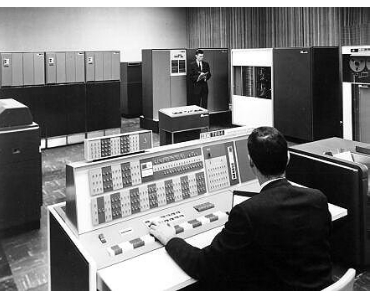
\includegraphics[width=.8\linewidth]{IBM7094.jpg}
  \end{sidecaption}
\end{figure}

En parallèle du perfectionnement des machines et de leur puissance de calcul apparaissent des langages de programmation qui vont faciliter la construction et la diffusion des méthodes de simulation. Nous n'envisageons pas d'en faire un historique complet, mais nous en donnons un aperçu dans l'encadré \enquote{Les premiers langages de programmation}.

D'un point de vue technique \textcite{Haggett1969} cite comme véritable point de départ dans la discipline la démocratisation de l'accès à la ressource informatique après 1961, avec la diffusion d'une deuxième génération d'ordinateurs dans les grands centres de calculs, en partant notamment de la série IBM 7094, le \textit{Vogelback Computing Center} \Anote{vogelback_marble} ouvert en 1965 à Northwestern avec un CDC 3400 apparemment très vite complété avec la sortie du CDC 6400 (600 cartes perforées par minutes ! Une bonne occasion pour apprendre à utiliser correctement le matériel de perforation \autocite{Fisk2005}) sur lequel vont travailler des pionniers comme Duane F. Marble \Anote{marble_computer_historycdc}. 

\pagebreak

\begin{testiv}{Les premiers langages de programmation}{}

La période 1955-1965 est une période où la simulation est reconnue comme une méthode de résolution d'un certain nombre de problèmes difficilement tractables mathématiquement.\autocite{Nance1993, Ackoff1961}. Des programmes de développement visant à mettre en place des modèles de représentation, de description nécessaire et facilitant la construction de simulations se multiplient. Deux classes de langages informatiques vont voir le jour durant cette période, et vont continuer à se développer et à s'influencer chacune de leur côté jusqu'à encore aujourd'hui. D'une part, des langages de plus haut niveau apparaissent avec pour vocation de se positionner comme une alternative plus expressive que l'assembleur. Dans cette optique le premier compilateur FORTRAN apparaît en 1957,  Algol en 1958, Cobol en 1959, et Lisp 1958. Ces langages et leurs successeurs sont d'usage assez générique et permettent de décrire correctement tous types de programmes. Toutefois à l'époque de leur apparition ils sont d'accès relativement difficiles pour une personne non initiée, ce qui nous amène au développement sur la même période d'une deuxième catégorie de langages informatique, plus spécialisé dans la construction spécifique de modèle de simulation. \autocite[239]{Naylor1966}

A la même époque, des langages spécialisés dans l'expression des simulations apparaissent, et pour la plupart s'appuient et évoluent en parallèle des développements des langages classiques sur lesquels ils s'appuient. Ces SPL ( \foreignquote{english}{Simulation Programming Langages}) comme Simula en 1962 ou bien Dynamo en 1958 ont ceci d'intéressant qu'ils ont très largement accompagné les formidables avancées conceptuelles de cette époque et cela au travers des différentes disciplines. Ainsi la première période 1955-1960 est marquée par la mise au point de GSP (\foreignquote{english}{General Simulation Program}) par Owen et Tocher \autocite{Tocher1960}. Celui-ci est considéré comme le tout premier langage mis au point pour faciliter la description de simulation sur ordinateur. Un effort que Tocher va accompagner d'une publication phare en 1963 dans le livre \foreignquote{english}{Art of Simulation} \autocite{Tocher1963} . Vient ensuite une autre génération de langage en 1960-1965 comme GPSS (\foreignquote{english}{General Purpose System Simulator}), Simscript (développé sous l'impulsion de la RAND corporation), et la première version du langage SIMULA, qui donnera naissance à la fin des années 1960 à Simula-67, un langage qui aura un impact dépassant largement la classe des SPL, et inspirera les créateurs des futurs langages objets comme Alan Kay, plus connu comme le créateur du premier langage objet SmallTalk. 

%% FIXME ORTHOGRAPHE DEUX PARAGRAPHE CI DESSOUS
On trouve plus d'informations sur cette période spécifique abordée sous l'angle de l'ingénierie logicielle dans les publications de \textcites{Nance2013,Nance1993, Araten1992, Nance2002} et en consultant les \href{http://informs-sim.org/}{@archives} de la WSC (\textit{Winter Simulation Conference}). Cette dernière, si elle n'est pas la première à aborder cette thématique (le \textit{System Simulation Symposium} en 1957 selon Nance), est la première à vouloir pérenniser le débat à un niveau national \autocite{Nance2002}. Fondée en 1967 \autocite{Crain1992, Araten1992} celle-ci jouit aujourd'hui d'une très large visibilité au niveau international, notamment car elle abrite les publications de pionniers et de membres importants pour la discipline simulation. On pourra citer par exemple Sargent et Balci, des pionniers dans la construction de la discipline de la \textit{Validation \& Verification}, qui participent et publient régulièrement dans le cadre de cette conférence. 

Les \textit{procedings} de la conférence WSC accueille ces dernières années le récit d'un projet réunissant un grand nombre d'acteurs importants pour l'émergence de la simulation \autocite{Nance2013}. Une fondation créée pour cette occasion est chargée de la récolte des témoignages audio et vidéo, de leurs préservations et de leurs mises à disposition avec tous les documents initiaux fondateurs sur le \href{http://d.lib.ncsu.edu/computer-simulation/}{@Computer-Simulation-Archive} hébergé par la \textit{North Carolina State University}

\end{testiv}


Des ordinateurs que l'on imagine beaucoup plus accessibles et performants que la précédente série IBM 604 et 650 \Anote{tobler_650} \autocite[584]{Barnes2004} à \textit{vacuum tube} utilisés au début des années 1960 à l'université de Washington \Anote{ibm604650} et Iowa, des précurseurs qui seront rapidement remplacés, par exemple par l'IBM 1620 enfin utilisable avec le langage Fortran I \autocite[66]{Berry2005}. 

%DEBUT ORTHOGRAPHE EMILIE
\hl{CORRECT JUSQUE FIN}
En Grande Bretagne, en 1951 il y aurait 4 ordinateurs seulement. En plus des universités déjà pionnières (Edinburgh, Londres, Oxford, Cambridge) et sous l'impulsion du \textit{Flowers Report} les universités s'équipent progressivement à partir du milieu des années 1960 suivant ce plan établi nationalement. On trouve un peu partout dans les universités \Anote{atlas} un motif assez similaire à celui de l'université de Bristol décrit par \textcite{Haggett1969}, c'est à dire une hiérarchie de machines qui va par ordre croissant de puissance de l'IBM 1620 et PDP 8 (Faculty level), l'Elliott 503 (University level), English Electric System 4-75 (South West Regional Computer Centre). Viennent ensuite les machines plus souvent remplacées des différents centres de traitements nationaux comme le \textit{SRC Atlas Computing Centre} de Chilton, le \textit{National Computing Centre} de Manchester, et bien d'autres centres plus petits, la plupart du temps accessibles à distance aux universitaires par divers terminaux. \textcite{Rhind1989} témoigne de la présence à l'université d'Edinburgh en 1967 d'une \textit{English Electric System KDF9} de puissance probablement similaire à celle évoquée par Haggett à Bristol. Depuis 1969 et jusqu'à 1973, soit un an à peine avant la commercialisation des tout premiers \textit{microcomputers}, \foreignquote{english}{The most sophisticated computing system in British universities was the NUMAC one, serving the whole of the universities of Newcastle and Durham: this IBM 360/67 had 1 Mb of main memory.} \Anote{numac} Un 360/65 est également installé la même année à l'\textit{University College} de Londres.

La mise en perspective de ces machines anglaises avec les travaux des géographes Ward et Weeb est intéressante. Ceux-ci se sont associés à l'informaticien Levison pour concevoir et exécuter des simulations spatiales de type Monte-Carlo pour étudier les théories de peuplement de la Polynésie, en utilisant l'ordinateur ATLAS, entre 1964 et 1971 \autocites{Montillier1974, Ward1973}. Cette expérience est régulièrement citée par \textcites{Gould1970, Gould1975} comme un autre des usages pionniers mêlant une discrétisation spatiale, un tirage Monte-Carlo, et une représentation des résultats sous forme de carte.

\foreignblockquote{english}[\cite{Gould1970}]{Handling space and time simultaneously is a difficult business, and simulation, for all its current detractors, often appears to offer the only feasible way out. [...] In an intriguing study of Polynesian drift voyaging, over 800000 items of data had to be stored in the computer’s memory before the Monte Carlo process could even begin [...] The model generated starting islands, and then simulated the drift voyages by drawing from probability distributions assigned to each five degree grid cell in the Pacific Ocean.}

\foreignblockquote{english}[\cite{Doran1974}]{ By use of computer techniques the authors have simulated an enormous number of voyages in the Pacific, over 100,000 drift voyages and about 8,000 guided voyages [...] Results of the various experiments are displayed on a series of maps showing probabilities of contact among islands, both by drift and by navigated voyages. An appendix reproduces eighty-four computer maps, each from a single experiment, which show the position of each vessel on each day of the many voyages. As many as 50,000 dots are shown on each map, providing an excellent visualization of the field covered by the experiment.}

%FIN ORTHOGRAPHE EMILIE

En Nouvelle-Zélande, Golledge nous indique que l'installation sur le territoire de la firme IBM semble précéder de peu la formation des pionniers \autocite[94]{Bailly2000} et au début des années 1960 l'université de Canterbury se porte acquéreur d'un flambant neuf IBM 1620 doté de 32K de mémoire.\Anote{ordinateur_actuel}

\Anotecontent{histoire_suede}{Une récolte de documents publique nationale a été organisé par le \textit{tekniskamuseet} de Suède, les textes sont disponibles à l'adresse internet suivante \href{http://www.tekniskamuseet.se/it-minnen}{@tekniskamuseet}}

En Suède \Anote{histoire_suede}, trois ordinateurs sont construits dans le courant des années 1950-1960 : SARA par la société Saab à Linköping, DASK à l'institut scientifique de Copenhague, et SMIL à l'université de Lund \autocite{Persson2007}. Carl Erik Frödberg, un ami d'enfance de Hägerstrand, fait partie avec Eric Stemme des consultants amenés à échanger sur le sol américain avec les leaders du domaine (Neumman, etc.) afin de démarrer le programme suédois.  SMIL est capable de compiler de l'Algol, et c'est probablement sur celui-là que Hägerstrand assisté de Frödberg a pu exécuter ses premiers programmes. En 1969, un Univac 1108 est acheté pour faire suite à SMIL \autocite[33-34]{Lindgren2008}.

En France, en 1955 il y a exactement six ordinateurs \autocite[3]{Armatte2008}, mais c'est seulement en 1970 que l'université Paris 1, centre de référence pour les géographes pionniers quantitativistes, se dote d'un ordinateur Philips et d'un terminal en contact avec le calculateur d'Orsay. Nous verrons plus en détail la relation historique des géographes aux centres de calculs dans la section \ref{sec:retourgeoHPCopenmole}.

Toutefois, on ne peut parler d'une véritable démocratisation de l'outil informatique chez les chercheurs qu'avec l'apparition dans les années 1974 aux États-Unis des premiers postes informatiques individuels \autocite[221]{Ceruzzi2000} et il faudra encore attendre le milieu des années 1980 pour que cette technologie se diffuse véritablement et touche le grand public.

A cette période la mise en oeuvre de modèles de simulation est fortement limitée par des problématiques humaines et techniques \autocites{Haggett1969}[387]{Marble1972}, dont on peut constater dans les ouvrages interdisciplinaires vus dans la section précédente, qu'elle ne touche pas en réalité que la géographie \autocite{Guetzkow1972}.

C'est toutefois dans cette période où les compétences informatiques nécessaires à la programmation se font encore très rares, les langages de programmation multiples et peu stables, le matériel coûteux et peu disponible (nécessitant des opérateurs de saisie, temps d'utilisation partagé entre différentes disciplines, accessible seulement localement), que des packages de programmes sont peu à peu publiés et mis à disposition des chercheurs via les réseaux universitaires \autocite{Haggett1969}. 

Au niveau de ces réseaux de diffusion de programmes, selon \textcite[20-21]{Greer1972} deux sont à noter : \textit{the State Geological Survey of University of Kansas (Computer Contributions)}  et \textit{ the Department of Geography of the University of Nottingham U.K. (Computer Applications in the Natural and Social Sciences)}. Au niveau des progiciels, \textcite[20-21]{Greer1972} identifie en 1972 trois pôles universitaires importants : Iowa \autocite{Wittick1968}, Northwestern \autocites{Marble1967, Marble1972b, Marble1972,Marble2010}, Michigan \autocite{Tobler1970c} \Anote{programme_trouver}. En effet, des pionniers comme Marble ou Tobler mettent à disposition dans le courant des années 1960 différentes routines informatiques en libre accès, \textcites[3]{Marble1967, Pitts1968} parle de 150 routines développées jusqu'à 1967, et cela seulement à Northwestern dans le département de géographie. Le premier \textit{Statistical package for Social Science} pour les sciences sociales (ou \href{http://www.spss.com.hk/corpinfo/history.htm}{@SPSS}) date quant à lui de 1968 \autocite{Barnes2011}, alors que sort à la même date l'ouvrage \foreignquote{english}{best-of} de \textcite{Berry1968} \foreignquote{english}{Spatial Analysis: a Reader in Statistical Geography}, qui offre une vision d'ensemble des derniers développements statistiques et mathématiques.

En faisant régulièrement état de leurs avancements dans divers rapports ou publications\Anote{programmes}, les pionniers Marble, Morrill, Pits et Bowlby \autocite{Pitts1963} qui se placent dans la continuité des premiers travaux relatifs aux processus de diffusion d'Hägerstrand \autocite{Hagerstrand1953, Hagerstrand1967a} donnent ainsi à voir les efforts et les difficultés auxquelles la petite équipe doit faire face pour améliorer les programmes ou les adapter à des problématiques différentes.

Sur un tout autre front, celui du développement des \textit{Large Scale Models} \autocites[8]{Batty1976}, les universitaires géographes sont plus souvent cités comme spectateurs qu'acteurs \autocites[9]{Batty1994}[153]{Batty1989}, cela même si quelques universitaires arrivent à décrocher des contrats importants \autocite{Barnes2006a} pour des études plus pratiques, comme \textcite{Garrison1959}, notamment du fait que les objectifs poursuivis sont relativement différents, la planification et la prédiction prenant plus souvent le pas sur la curiosité et l'explication scientifique. Toutefois, et si on en croit \textcite{Haggett1969} la communauté universitaire semble attendre beaucoup des retombées de ces grands programmes, qui disposent de moyens humains et économiques importants pour développer des programmes et collecter des données. Cette crise, qui on l'a vu touche avant tout les instituts de planification américains couverts par la RAND, va fournir le terreau nécessaire à la transformation d'une discipline dont le rayonnement dans la communauté scientifique à l'international ne va aller qu'en s'amplifiant après 1970 (voir la carte \ref{fig:S_carte_wegener}).

\begin{figure}[h]
\begin{sidecaption}[fortoc]{La carte des centres de recherches les plus actifs à la fin des années 1980, début des années 1990 selon \textcite{Wegener1994}}[fig:S_carte_wegener]
  \centering
 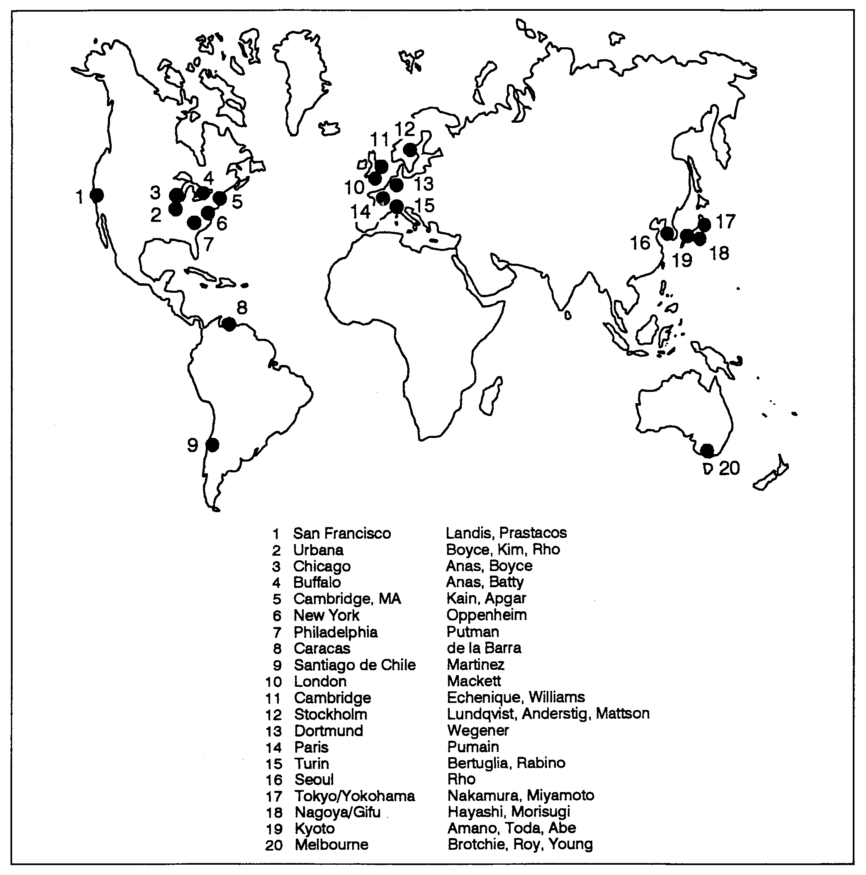
\includegraphics[width=.9\linewidth]{carte_wegener.png}
  \end{sidecaption}
\end{figure}

Si le requiem de \textcite{Lee1973} a bien eu un effet non négligeable sur la construction et la publication de tels modèles du coté des planificateurs \footnote{Seulement trois modèles seront publiés dans le même journal à la suite de cet article ...}, force est de constater que la construction de modèles de simulation pour la théorie urbaine ne disparaît pas dans cette période \autocite[11-12]{Batty1994}, et s'appuie au contraire sur l'apprentissage de ses échecs pour se réinventer dans les années qui suivent. A ce titre, \textcite{Harris1994} soulève dans une relecture très critique de l'article de Lee, l'ignorance ou la méconnaissance de l'auteur vis-à-vis des débats qui agitent déjà depuis plusieurs années la simulation de modèles urbains \autocites{Batty1971, Wilson1970, Orcutt1957, Harris1968}. Ce faisant, Harris accuse Lee d'enfoncer des portes ouvertes et de porter des accusations que certains jugeront par la suite prématurées vis-à-vis du préjudice subi, touchant à cœur une discipline d'à peine une décennie et encore en phase d'apprentissage. \autocite[p11]{Batty1994}.

Ce mouvement de modélisation doit faire face à l'expression de ces limitations pour se reconstruire, limitations dont on sait par avance qu'elles ne seront pas seulement levées par la seule amélioration des techniques.  

D'une part l'emploi de théories trop simplistes, induit indirectement la nécessité d'un retour à une démarche inductive plus exploratoire \footnote{On notera par exemple le témoignage de \textcite{Boyce1988} lorsqu'il dit à propos des chercheurs engagés dans cette voie \foreignquote{english}{Some, including myself, turned to more empirically oriented research activities, perhaps in the hope of strengthening the foundation of future models}}, jusque là mise de coté. \hl{On peut ici aussi ajouter la référence aux différents articles de l'ouvrage anniversaire (20 ans apres model geography) Remodelling Geography de MacMillan en 1987}

D'autre part, si les universitaires américains semblent rater le coche de cette transformation, en Europe plusieurs écoles viennent à se former, et intègre les défauts et les qualité de cette génération précédentes de modèle. C'est le cas par exemple au Royaume-Uni où sont récupérés les modèles américains ayant donné de bons résultats, comme celui de Lowry \autocite{Lowry1964}, pour servir de base à de nouveaux travaux mettant en perspective l'influence ou les progrès d'autres courants disciplinaires en contact avec la géographie. Car une autre voie d'évolution possible pour les modèles vient des travaux existants réalisés dans d'autres disciplines universitaires ou dans le monde industriel. Ainsi différentes équipes de développements sont déjà bien identifiées dans la communauté des économistes comme \textcite{Orcutt1957} et son premier modèle micro \foreignquote{english}{bottom-up} développé à l'\textit{Urban Institute}, et l'apport de \textcite{Forrester1961,Forrester1969} sur l'optimisation industrielle, une des branches opérationnelles d'inspiration la plus directe du projet systémique au début des années 1960 \autocites{Cohen1961}[911]{Shubik1960b}. Ces deux exemples font dans leur implémentation dynamique alors écho aux travaux initiaux du géographe Hägerstrand, et poussent dans cette période de reconstruction toute une partie des géographes à réintégrer la dimension temporelle à des modèles d'optimisation statique en échec \autocite[p295]{Batty1976}.

\pagebreak

% et Hagerstrand ?
\begin{testiv}{La diffusion de la micro-simulation}{}

La \enquote{micro-simulation} initiée par Orcutt, qui semble effectivement passer outre l'extinction annoncée par Lee en 1973, rencontre même un certain succès durant toutes les années 1970 comme en témoigne la mise en place de nombreux programmes nationaux au début des années 1980 \autocites{Merz1991, Merz1994, Baroni2007}. Comme l'indique également \textcite{Boman2005} en citant \textcite{Merz1991} : \foreignquote{english}{[...] 57 major dynamic and static microsimulation models had been developed and implemented between 1960 and 1990. They covered the following topics: wealth accumulation and distribution, labor force participation, pension reform, family formation, distributional effects of tax transfer policies, urban housing markets, distributional impact of energy policies, national health insurance, state unemployment insurance, land-use forecasting, residential energy demand, housing allowance, labor supply, shortening of working hours, distributional impacts of child allowance changes, market and non-market activities, shadow economy, effects of tax regulations on industrial firms, and more.}

Une réponse à cette survie peut être avancée dans le positionnement innovant d'Orcutt pour faire face aux résultats décevants des \textit{Large Scale Models} de son époque, opérant pour la plupart à un niveau macro et fournissant des résultats hautement agrégés difficiles à exploiter dans un cadre prédictif, et finalement peu représentatifs de la diversité des systèmes économiques \autocites{Birkin2012, Baroni2007}. Si les critiques de Lee peuvent pour la plupart être mobilisées pour critiquer les modèles issus de la micro-simulation (complexité des modèles, absence d'objectifs clairement posés, volume des données à mobiliser, complexité des calculs, coût de construction, absence de résultats, etc.), il n'en reste pas moins que la proposition d'Orcutt introduit avec une approche plus \textit{bottom-up} une dimension explicative absente jusque là. En répondant à l'observation de Lee sur l'absence d'extraction de connaissances micro quelque soit la complexité injectée dans les modèles macro, Orcutt ouvre d'une certaine façon la voie à des développements théoriques beaucoup plus riches que ne le permettaient à l'époque les seuls modèles macro, faisant ainsi de son modèle un instrument réceptacle idéal pour accueillir des élements de complexification issues des sciences sociales \autocite[19]{Czajka1993}. Un travail pour \foreignquote{english}{consolidating past, present, and future research efforts of many individuals in varied areas of economics and sociology into one effective and meaningful model; an instrument for combining survey and theoretical results obtained on the micro-level into an all-embracing system useful for prediction, control, experimentation, and analysis on the aggregate level} \autocite[122]{Cohen1961}.

D'un autre coté, cette micro-simulation telle que déjà théorisée par Hägerstrand dans sa version spatiale ou par Orcutt dans sa version économique, va étonnamment et cela pendant plusieurs années rester un courant ayant peu d'impact sur le développement des modèles urbains en économie spatiale \autocite[5]{Sanders2006}, et cela malgré plusieurs appels d'un coté \autocite{Hagerstrand1970} ou de l'autre \autocite[5]{Isard1998}. De façon indépendante et dans un univers somme toute limité par de fortes contraintes techniques et financières, ces travaux vont toutefois dans leurs lentes et multiples convergences donner naissance autant à des modèles universitaires qu'à des programmes nationaux (DYNASIM et CORSIM pour Orcutt aux Etats-Unis, SVERIGE en Suède, etc.). Pour finir cette parenthèse sur la micro-simulation par une petite transgression temporelle, si peu de modèles existent encore dans les années 1990, plusieurs publications récentes font état d'un inversion de la tendance ces vingt dernières années \autocite{Lenormand2013}, avec une augmentation (et une diversification ? ) croissante des modèles, sûrement liée à des capacités de développements informatiques plus importants, tant du point de vue des données, que de la puissance d’exécution qui admet l'importance croissante du parallélisme, idéale pour simuler des entités individuelles. \autocites[5]{Sanders2006}{Lenormand2013}

\end{testiv}

D'autres écoles apparaissent dans le courant des années 1970, comme celle de \textcite{Wilson1970} dont l'émergence est considérée comme un des moment important dans le renouveau des modèles urbains \autocite{Griffith2010}; mais également d'autres écoles comme celle de Peter Allen, qui s'appuient sur l'évolution des mathématiques et le transfert méticuleux de concepts observés en physique pour construire des modèles à la fois spatiaux et dynamiques capables de simuler de façon plus réaliste les interactions complexes intervenant dans la formation et l'évolution des villes \autocites[11]{Batty1976}{Batty2001}[27-28]{Pumain2003} \Anote{pumain_gain}.  

La diffusion et la généralisation du \enquote{projet systémique} de Bertalanffy dans de multiples disciplines permettent aux géographes d'accéder à tous les outils conceptuels et surtout opérationnels \autocite{Forrester1969} nécessaires pour penser, modéliser et simuler les systèmes géographiques au travers de leurs interactions complexes, en intégrant dans leurs analyses cette hétérogénéité d'échelle caractéristique des objets géographiques, comme peut l'être par exemple la région. 

Ainsi pour \textcite[11]{Batty1976}, de façon plus importante que tous les autres problèmes, c'est la révélation dans l'observation de cette richesse et de cette complexité d'interactions des facteurs causaux à l’œuvre dans l'évolution et la structuration des phénomènes urbains qui va le plus contribuer à la réévaluation des formes de modélisation. Révélé par Batty comme le problème de l'\textit{Observational Dilemna} \autocite[11,296]{Batty1976} \Anote{observational_dilemna}, celui-ci s'impose à la fois comme un constat faisant suite à cette première génération de modèle \Anote{problem_generation_model} et une conséquence de cette prise en compte nécessaire de la \enquote{dynamique} dans les futurs modèles de simulation \Anote{batty_dynamic}. Tout en restant critique sur les capacités de celui-ci, c'est le modèle de Forrester \textit{Urban Dynamics} \autocite{Forrester1969} qui cristallise selon \textcites{Batty2001, Batty2005b} le mieux cette transformation dans la façon de penser la construction et la validation des modèles de simulation urbains au début des années 1970 \Anote{observational_validate}. 

Nous aurons l'ocasion de revenir plus en détail sur cette décennie charnière (section \ref{ssec:transition_annee70}) en abordant tout à la fois le glissement progressif de la géographie dans une pensée systémique et son impact sur les écoles anglaises et françaises de modélisation (section \ref{sssec:progressive_systemique}), jusqu'à évoquer plus concrétement cette \enquote{problématique de la Validation} au travers des arguments croisé de Forrester et de Batty (section \ref{sssec:forrester_impact}).

\subsubsection{De fortes limitations techniques et méthodologiques}
\label{ssec:limitation_techniques_methodologiques}

Dans la lignée des témoignages de \textcite{Marble1972} \Anote{marble_validation}, les modèles spatiaux restent selon \textcite{Batty1976} \Anote{limitation_batty} encore très limités dans leurs complexifications, ou même leurs évaluations compte tenu des ordinateurs à disposition des géographes. 

Malgré les apports heuristiques indéniables qui vont avec l'utilisation de l'outil, on retrouve l'expression de difficultés concernant le calibrage des modèles plus complexes chez de nombreux auteurs pionniers modélisateurs \autocites{Batty1976,Pumain1983b}[400]{Sanders1984}, notamment pour ce qui concerne le calibrage des modèles, souvent difficile pour ces modèles dynamiques non linéaires soumis à de tels fluctuations dans leur comportements. Voici comment \autocite{Pumain1998a} résume les difficultés opérationnelles résultats de plusieurs années de travaux menés autour des modèles de simulation dynamiques non-linéaires opérant dans le cadre de la théorie de l'auto-organisation : \enquote{Les difficultés de calibrage, associées à la capacité élevée de bifurcation des modèles, ont été maintes fois décrites, de même que l’impossibilité de valider comme \enquote{meilleur ajustement} une configuration donnée de paramètres.}

Se pose alors la question suivante, l'incapacité à calibrer un modèle de simulation n'est-elle pas un problème qui limite de facto l'évolution en crédibilité de l'outil simulation ? 

On perçoit pourtant très tôt chez certains géographes la nécessité d'optimiser cette étape, rendue improductive et dangereuse du fait de la non-linéarité des modèles \foreignquote{english}{The trial and error method of searching for best-parameter values by running the model exhaustively through a range of parameter values or combinations thereof represents a somewhat blunt approach to model calibration. [...] Moreoever, as each run of the model can be expensive or take a large amount of time, few applications have attempted to find systematically the optimum parameter values [...] Clearly, then, there is a need for the introduction of methodes suitable for calibrating intrinsically non-linear models of spatial interaction.} \autocite[155]{Batty1976}

Des méthodes basées sur des méta-heuristiques de type descente de gradient, ou \textit{hill-climbing} sont déjà utilisées par les géographes comme \textcite[159-160]{Batty1976} pour résoudre des problèmes d'optimisations utilisant les sorties de modèles. Toutefois ces méthodes sont encore trop souvent limitées à des modèles à 1 ou 2 paramètres, s'avèrent peu robustes face à des problèmes acceptant des minima locaux, et se limite à l'optimisation de fonctions uniquements unimodales. Les équipes françaises se heurtent également à ces problématiques au début des années 1980, et ces nouveaux modèles \enquote{complexes} restent très difficile à calibrer avec les moyens informatiques disponibles, même lorsque ceux-ci sont importants \autocites{Pumain1983b, Sanders1984}.

A cela vient s'ajouter une autre problématique. En effet, à l'inverse des pionniers géographes français qui manifestent très tôt la volonté d'une modélisation en confrontation avec l'empirie \autocites{Pumain1983,AMORAL1983}, \textcite{Openshaw1989} formule à la fin des années 1980 quelques critiques sérieuses à l'égard d'un mouvement de modélisation anglo-saxon qui se serait replié dans la production de modèles essentiellement mathématiques et théoriques \Anote{end_mathematical_area}. La prise en compte lucide de la complexité des systèmes urbains et de l'impossibilité d'en observer ou d'en recolter de façon simple la substance causale (\textit{observational dilemna}) ne doit pas masquer la nécessité d'une confrontation pratique avec les données, ne serait ce que pour nourrir en retour les constructions théoriques. Si Batty en est bien conscient, ce n'est pas semble-t-il le cas de tout un courant de modélisateur anglo-saxon à cette époque. \textcite{Openshaw1989} nous dit également que cette \enquote{problématique de la Validation} n'a pas toujours été abordée de façon concrète \Anote{openshaw_critique_math}, par le spectre d'outils ou de méthodes susceptible d'être mis à disposition des modélisateurs. L'absence dans la littérature de logiciels, de codes sources, ou de réelle méthodologie pour la construction ou l'évaluation des modèles de simulation face aux données reste selon \textcite{Openshaw1989} un frein à toute adoption plus large de cette activité de modélisation. Comme le laisse aussi supposer le titre du chapitre 1 de \textcite{Batty1976} \textit{The art of urban modelling}, construire des modèles reste à cette période une activité dont \enquote{les rouages informatiques} sont bien gardés. %En france aussi

L'appel à l'utilisation de nouvelles méthodes pour l'exploration des modèles déjà lancés par \textcite{Batty1976} sera par la suite repris de façon implicite dans les travaux innovants mené par l'équipe de géographes de Leeds, principalement guidé par l'inventivité d'Openshaw \autocites{Openshaw1983, Openshaw1988, Diplock1996, Turton1998}. Celui-ci publie par exemple avec \textcite{Diplock1996} un des premiers article sur les algorithmes génétiques utilisé pour estimer des paramètres de valeurs inconnu lors des calibrages de différents modèles spatiaux :

\foreignblockquote{english}[\cite{Diplock1996}]{The results demonstrate that even GA en ES can provide very good solutions for spatial interaction model calibration, albeit sometimes at the expense of considerable extra compute times. [...] It would also be worth considering the use of other forms of global optimization method; [....] As computer hardware becomes faster, the attraction of simple, relatively assumption-free, and highly robust approaches to global parameter estimation can only grow and allow the geographical model builder to worry less about the problems of parameter estimation and focus more on the task of model design.}

Remis en perspective de l'\textit{observational dilemna} de Batty, la dernière phrase d'Openshaw prend alors tout son sens. La possibilité d'une telle systématisation dans le calibrage des modèles permet au modélisateur de se concentrer sur le seul vrai débat censer rythmer la construction des modèles de simulation, à savoir la selection et la justification des hypothèses que l'on veut intégrer dans la structure causale de nos modèles de simulation. Avec de tels outils s'appuyant sur des puissances de calcul intensive bien au delà de ce que permet un micro-ordinateur, la dépendance des modélisateurs à la ressource informatique se renforce en réalité encore un peu plus dès lors qu'on considère la nécessité d'explorer les modèles, non plus lorsqu'ils sont terminés, mais dès que la première brique est posée. 

Cette réponse plus méthodologique et technique à \enquote{la problématique de la Validation} sera discutée (section \ref{ssec:evaluation_construction}) à la fois dans ses implications épistémologiques (explorer ainsi les modèles de simulation est-il suffisant pour dire de ceux-ci qu'ils sont validés ?) mais également dans ses implications plus concretes, dans le cadre d'une évolution des pratiques de modélisation au laboratoire Géographie-cités (partie 2 de la thèse).

\subsection{Synthèse}

%%FIXME PAGE REF DYKE

Il semblerait donc que la pratique de la simulation en sciences sociales se concentre ensuite dans les années 1980 sur de petites communautés de chercheurs, disposant de fortes compétences techniques initiales, qui vont continuer à travailler, à proposer des modèles et à acquérir de nouvelles techniques et méthodologies en parallèle d'un courant plus \textit{mainstream} intégrant seulement les nouvelles capacités offertes par les ordinateurs mais délaissant parfois l'aspect simulation. Dès les années 1980-1990, plusieurs chercheurs pionniers, comme Jim Doran \autocites{Doran1982, Doran1986}, réapparaissent conjointement avec l’avènement d'une nouvelle innovation dans les techniques de simulation en partie dérivée des progrès en intelligence distribuée; un retour dont on verra qu'il se fait cette fois-ci avec plus de succès.

En s'appuyant sur ces livres interdisciplinaires déjà cités de multiples fois \autocite{Dutton1971,Guetzkow1962, Guetzkow1972} et sur ce qui a été dit dans ce chapitre, voici une liste forcément non exhaustive d'arguments évoqués par les auteurs pour justifier de cette baisse effective dans la confiance envers l'utilisation des modèles de simulations : \textbf{(1)} l'effet de mode initial qui exagère largement les capacités de l'outil pour expliquer ou prédire \textbf{(2)} les effets négatifs d'un rattachement volontaire ou involonaire à l'idéologie néo-positiviste, un programme épistémologique vivement critiqué durant les années 1970 dans plusieurs disciplines des sciences sociales, \textbf{(3)} la non-adéquation entre la richesse d'expression des théories sociales et la concision/réduction mathématique, \textbf{(4)} l'absence de standard de validation prenant en compte le cadre thématique, voire l'absence complète de validation, \textbf{(5)} la non-adéquation avec un courant théorique \textit{mainstream} réfractaire, \textbf{(6)} les capacités encore limitées des ordinateurs de l'époque, pour le stockage des données, pour l'exécution des programmes, pour l'exécution des analyses sur les modèles, et pour les réplications nécessaires à la validation, \textbf{(7)} l'ignorance ou la difficulté à mettre en oeuvre les techniques adéquates, va de pair avec le manque de formation/compétence pour ces nouveaux outils dans la discipline, et rend difficile l'exploitation et la construction des modèles, \textbf{(8)} l'existence de parcours et de stratégies de publications scientifiques non adaptés pour ce nouvel objet de recherche qui limite sa diffusion : concentration sur les seuls résultats du modèle, peu ou pas de suivi dans l'évaluation des modèles sur le long terme.

Certains arguments sont clairement conjoncturels, beaucoup se recoupent, et d'autres englobent toutes les dimensions, comme la \enquote{problématique de la Validation} dont on a vu qu'elle aborde finalement des questions de fond sur tous les plans : technique, méthodologique, philosophique et institutionnelle. %\hl{Pour herman, voir Padioleau p209 p205, + scepticisme de boudon, voir citation p205}

En pointant en géographie l'existence d'une transformation touchant \enquote{la pratique de la simulation} lors de son transfert des pionniers américains aux pionniers européens, nous espèrons ouvrir pour la suite un débat sur la Validation qui s'appuie lui aussi sur une réévaluation des pratiques de modélisations en regard des différents aspects intervenant dans cette problématique de la validation. % non plus uniquement sur les aspects technique mais également méthodologique.

Les chapitres suivants seront donc marqués par d'autres aller-retours entre passé et présent, afin de mettre en avant la persistance, ou la transformation de certains de ces points intervenant dans une problématique dont on peut déjà entendre en 1970 de la bouche des spécialistes, qu'elle sera un des problèmes les plus difficiles à résoudre dans le futur \autocites{Hermann1967, Naylor1967, Guetzkow1972, Doran1975}. 

%\textit{Dans quelles mesures les problématiques levées à la fin de la section précédente ( section \ref{ssec:disciplines_touches}) sont-t-elles encore pertinentes après une telle évolution des pratiques dans la géographie ? }

% TYPOLOGIE A REVOIR SUREMENT POUR MIEUX LA RANGER
